\myparagraph{
    In questo capitolo, vengono analizzati dei design pattern nuovi e non trattati
    durante il corso di Analisi e Progettazione.
    Verrà fatto anche qualche riferimento a pattern già visti.

    \begin{tcolorbox}[colback=red!5!white, colframe=red!75!black]
        \textbf{Attenzione}, il file fornito chiarisce solo le nozioni teoriche sui pattern trattati, per
        approfondirli in maniera pratica si consigliano le slide fornite dai professori (e ovviamente testare
        su codice il loro funzionamento).
    \end{tcolorbox}
}

\mysubsectionformatted{Design Pattern State}
\myparagraph{

    \begin{tcolorbox}[colback=blue!5!white, colframe=blue!75!black]
        Permette a un oggetto di modificare il suo comportamento quando il suo
        stato interno cambia.
    \end{tcolorbox}

    \noindent\textit{State} viene utilizzato quando si vuole modificare lo stato interno di un oggetto
    in modo da potergli far eseguire determinati metodi. Gli stati degli oggetti vengono rappresentati
    da classi differenti che estendono una classe astratta che rappresenta lo stato dell'oggetto.

    \begin{center}
        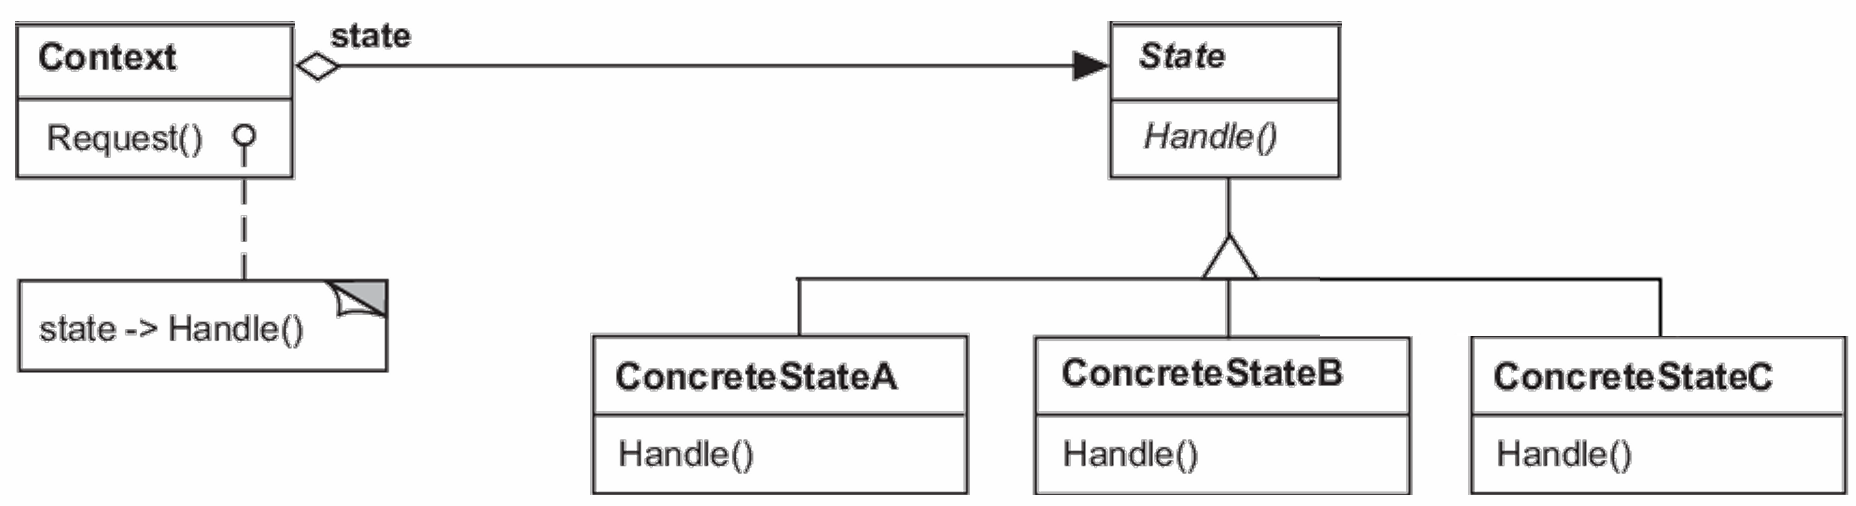
\includegraphics[scale=0.25]{Esercitazione - Design Patterns/state_pattern.png}
    \end{center}

    \begin{enumerate}
        \item \textbf{Context} è l'interfaccia del client. Ha un'istanza di \textbf{ConcreteState} che indica in che stato si trova.
        \item \textbf{\textit{State}} è la classe astratta che rappresenta lo stato attuale di \textbf{Context}.
        \item \textbf{ConcreteState} sono le classi che implementano il comportamento \\associato allo stato del \textbf{Context}.
    \end{enumerate}

    \begin{center}
        \resizebox{\columnwidth}{!}{%
            \begin{tabular}{|l|l}
                \hline
                \rowcolor[HTML]{32CB00}
                \multicolumn{1}{|c|}{\cellcolor[HTML]{32CB00}\textbf{Vantaggi}}                                                                       & \multicolumn{1}{c|}{\cellcolor[HTML]{FE0000}\textbf{Svantaggi}} \\ \hline
                Eliminazione di tanti "if"                                                                                                            & \multicolumn{1}{l|}{Incremento del numero di oggetti}           \\ \hline
                Facile lettura del codice                                                                                                             & \multicolumn{1}{l|}{Richiede la scrittura di molto codice}      \\ \hline
                \begin{tabular}[c]{@{}l@{}}Nuovi stati e transizioni possono essere\\ aggiunti facilmente definendo nuove \\ sottoclassi\end{tabular} &                                                                 \\ \cline{1-1}
            \end{tabular}%
        }
    \end{center}

    \newpage
    \subsubsection{Esempio di Pattern State}
    \begin{center}
        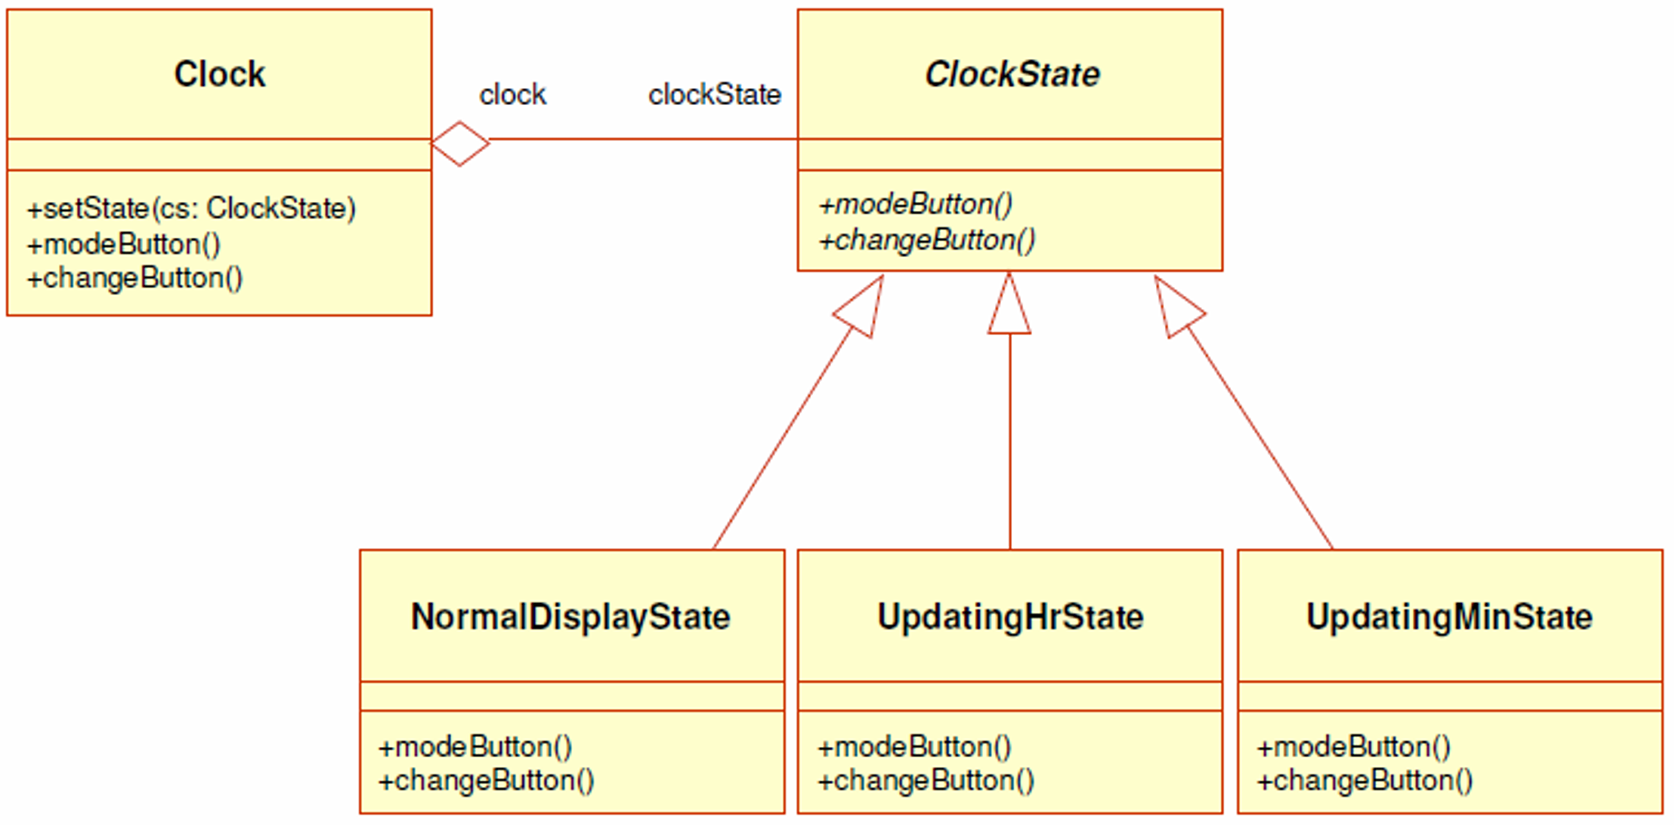
\includegraphics[scale=0.25]{Esercitazione - Design Patterns/example_state_pattern.png}
    \end{center}
    In questo esempio, \textbf{Clock} contiene 3 metodi di cui \textbf{modeButton()} e \textbf{changeButton()} cambiano il loro
    comportamento in base allo stato in cui si trova. \textbf{setState(cs: ClockState)} permette di cambiare lo stato di \textbf{Clock},
    in questo modo, anche i due metodi all'interno cambieranno il loro comportamento.

    \mysubsubsectionformatted{State vs Strategy}
    Sono entrambi pattern comportamentali, ma hanno obiettivi e applicazioni \\differenti.

    \begin{tcolorbox}[colback=blue!5!white, colframe=blue!75!black]
        State cambia il comportamento di un oggetto in base al suo stato interno.
        \\Es. Un lettore audio che può avere stati come "Play", "Pause" e "Stop", dove ogni stato 
        gestisce le azioni dell'utente in modo diverso.
    \end{tcolorbox}

    \begin{tcolorbox}[colback=green!5!white, colframe=green!75!black]
        Strategy consente di cambiare il modo in cui un'operazione viene eseguita, senza modificare lo stato interno dell'oggetto.
        \\Es. Un sistema di pagamento che può usare diverse strategie come "Carta di credito", "PayPal" o "Bonifico", a seconda della scelta dell'utente.
    \end{tcolorbox}
    \newpage

}

\mysubsectionformatted{Design Pattern Command}
\myparagraph{

    \begin{tcolorbox}[colback=blue!5!white, colframe=blue!75!black]
        Permette di trasformare una richiesta in un oggetto indipendente.
        \\In questo modo si possono:
        \begin{enumerate}
            \item scollegare il mittende di una richiesta dal destinatario.
            \item rendere le operazioni riutilizzabili.
            \item registrare e annullare operazioni.
            \item creare sequenze di comandi.
        \end{enumerate}
    \end{tcolorbox}
    \noindent\textit{Command} è ideale per implementare operazioni complesse e modulari
    che possono essere facilmente eseguite, annullate, memorizzate e organizzate in sequenza.

    \begin{center}
        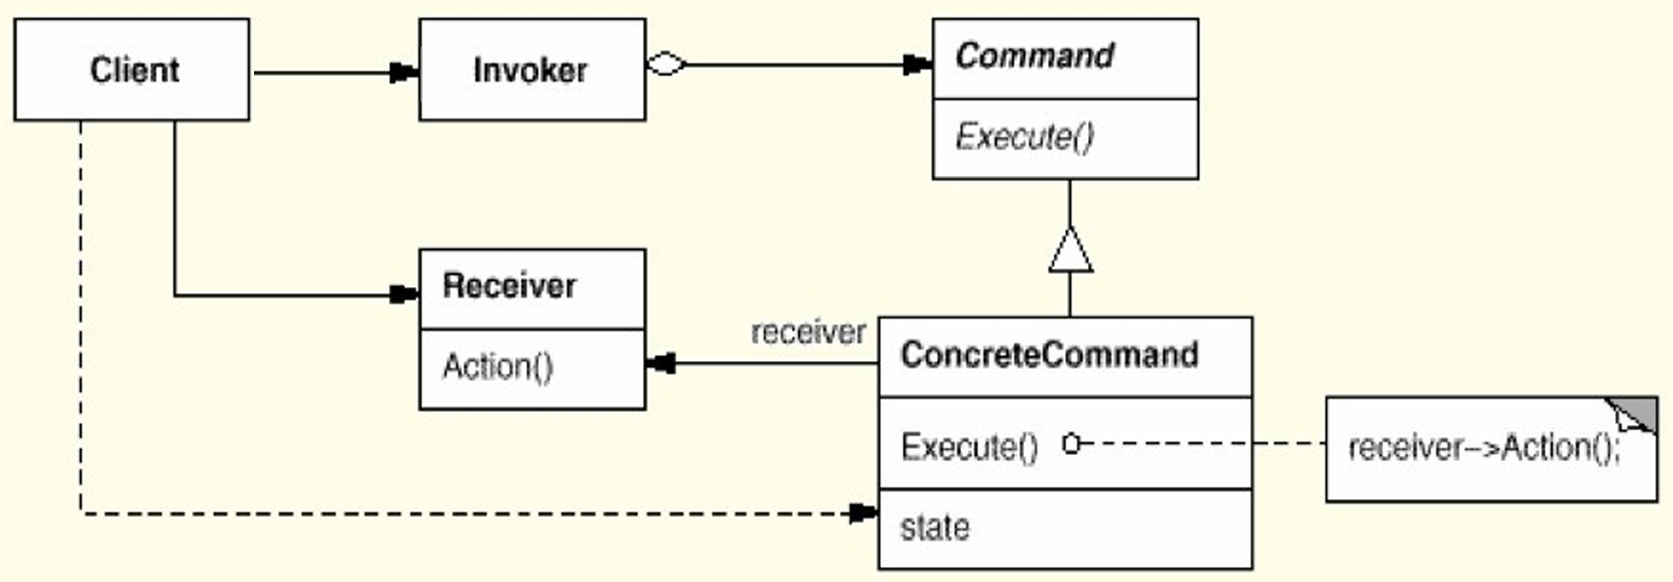
\includegraphics[scale=0.25]{Esercitazione - Design Patterns/command_pattern.png}
    \end{center}

    \begin{enumerate}
        \item \textbf{Client} è l'interfaccia che crea un'istanza concreta  \textbf{ConcreteCommmand}
              e ne imposta il \textbf{Receiver}.
        \item \textbf{\textit{Command}} è l'interfaccia per l'esecuzione dell'operazione.
        \item \textbf{ConcreteCommand} è la classe che incapsula l'operazione da eseguire
              in un oggetto specifico.
        \item \textbf{Invoker} è la classe che che richiede tramite il \textbf{\textit{Command}}
              l'esecuzione di una o più operazioni.
        \item \textbf{Receiver} è l'oggetto che esegue l'azione.
    \end{enumerate}

    \begin{center}
        \resizebox{\columnwidth}{!}{%
            \begin{tabular}{|l|}
                \hline
                \rowcolor[HTML]{32CB00}
                \multicolumn{1}{|c|}{\cellcolor[HTML]{32CB00}\textbf{Vantaggi}}                                                                                \\ \hline
                Separa l'oggetto che invoca l'operazione da quello che sa come eseguirlo                                                                       \\ \hline
                \begin{tabular}[c]{@{}l@{}}I \textit{Command} sono classi di oggetti e possono essere manipolati \\ come qualsiasi altro oggetto.\end{tabular} \\ \hline
                Si possono creare dei \textit{Command} composti.                                                                                               \\ \hline
                \'E semplice aggiungere nuovi \textit{Command}.                                                                                                \\ \hline
            \end{tabular}%
        }
    \end{center}
    \newpage
    \subsubsection{Esempio di Design Pattern Command}
    \begin{center}
        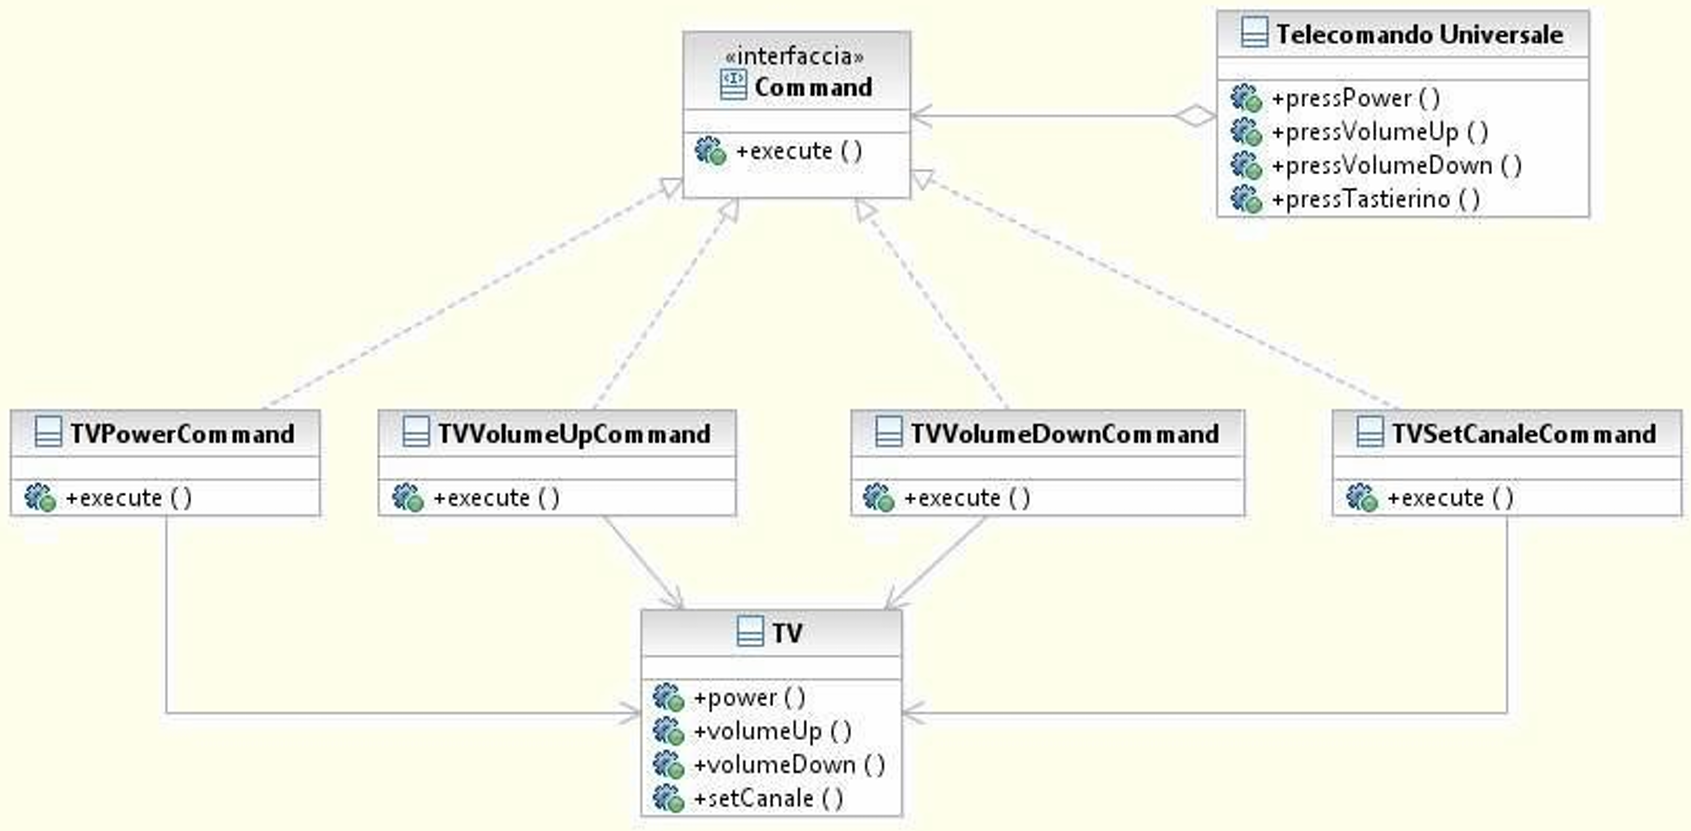
\includegraphics[scale=0.26]{Esercitazione - Design Patterns/example_command_pattern.png}
    \end{center}
    In questo esempio, \textbf{TV} è il \textbf{Receiver} che esegue l'azione stabilita dal \textbf{Telecomando Universale},
    ovvero l'\textbf{Invoker}. 
    \\
    I \textbf{ConcreteCommand} sono le 4 classi che ereditano il metodo \textbf{execute()} che
    invocano le corrispondenti operazioni del \textbf{Receiver}.
    \\
    Infine l'interfaccia \textbf{\textit{Command}} che definisce l'interfaccia alle classi concrete.
    \newpage

}

\mysubsectionformatted{Design Pattern Template}
\myparagraph{

    \begin{tcolorbox}[colback=blue!5!white, colframe=blue!75!black]
        Definisce lo scheletro in un'operazione, lasciando alle sottoclassi di \\modificare
        l'algoritmo senza cambiare la sua struttura.
    \end{tcolorbox}
    \noindent Usiamo \textit{Template} quando si vuole implementare le invarianti di un algoritmo una sola volta,
    saranno le sottoclassi a implementare le varie varianti.

    \subsubsection{Struttura del pattern Template}
    \begin{center}
        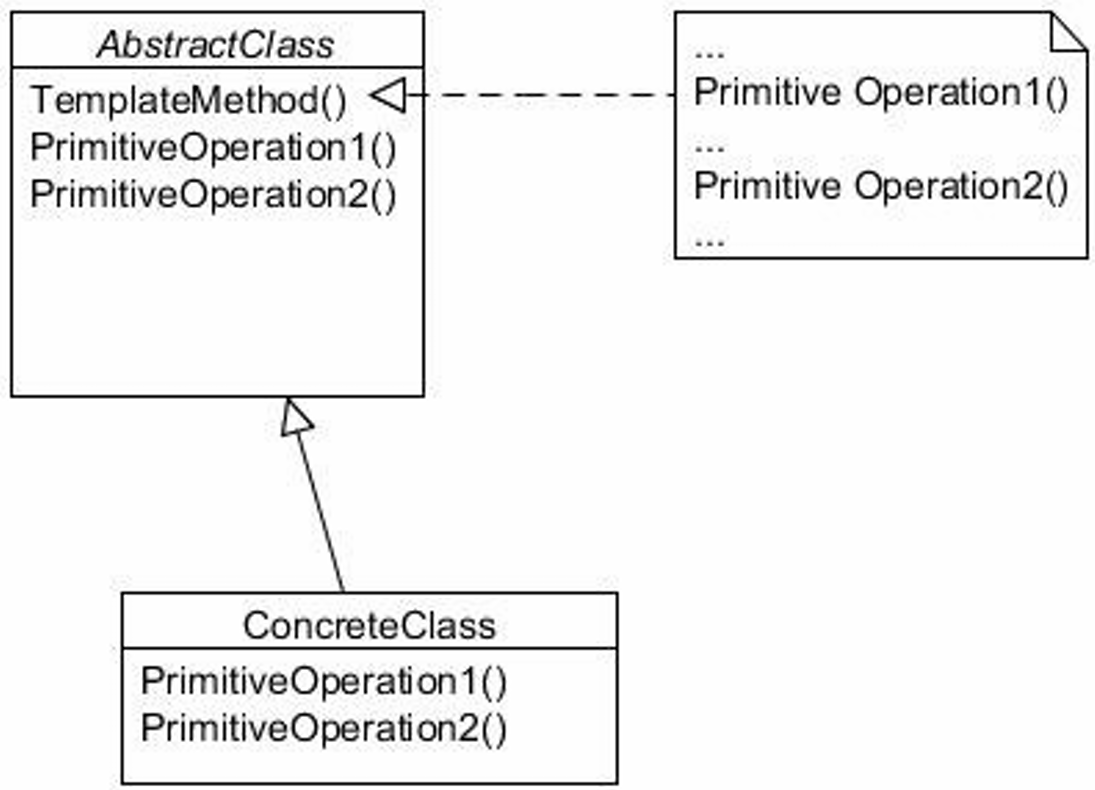
\includegraphics[scale=0.25]{Esercitazione - Design Patterns/template_pattern.png}
    \end{center}
    \begin{enumerate}
        \item \textit{\textbf{AbstractClass}} è la classe che definisce le operazioni primitive di tipo astratto.
        Queste vengono poi implementate dalle sottoclassi \textbf{ConcreteClass}. Definisce un metodo \textbf{TemplateMethod()}
        che rappresenta lo scheletro di un algoritmo e richiama le operazioni primitive.
        \item \textbf{ConcreteClass} sono le classi che implementano le operazioni primitive per poterne variare il 
        comportamento.
    \end{enumerate}
    I metodi template sono fondamentali per il riutilizzo del codice, soprattutto nelle librerie di classi, questo perchè
    sono i mezzi per estrapolare i comportamenti comuni in classi di libreria. Bisogna sempre specificare quali operazione 
    si vogliono sovrascrivere e quali metodi trasferiti alle sottoclassi.

    \newpage
    \subsubsection{Esempio di Design Pattern Template}
    \begin{center}
        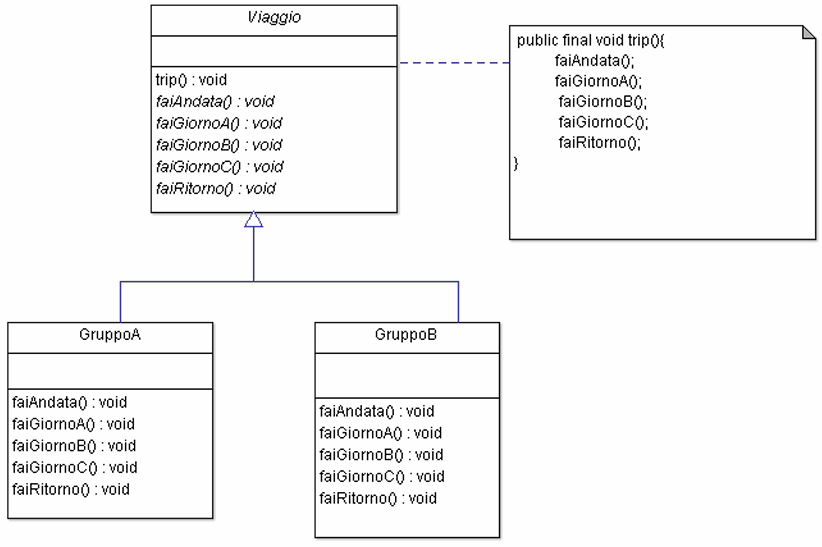
\includegraphics[scale=0.5]{Esercitazione - Design Patterns/example_template_pattern.png}
    \end{center}
    In questo esempio, \textit{Viaggio} è l'\textit{\textbf{AbstractClass}} che contiene il metodo Template \textbf{trip()}. Le
    \textbf{ConcreteClass} \textbf{GruppoA} e \textbf{GruppoB} ereditano i metodi dalla superclasse, decidendo però come deve essere
    implementato ciascun metodo.

    \newpage
}

\mysubsectionformatted{Design Pattern Repository}
\myparagraph{
    Questo design pattern viene usato se, ad esempio, si vuole accedere a una base di dati persistenti.
    
    \begin{tcolorbox}[colback=blue!5!white, colframe=blue!75!black]
        Il pattern fornisce un'illusione di una collezione in memoria per ogni tipo di oggetto persistente che
        richiede l'accesso globale. L'accesso avviene tramite un'interfaccia che definisce delle operazioni per
        aggiungere, rimuovere o ricercare oggetti. Queste operazioni incapsulano l'accesso effettivo alla rappresentazione
        dei dati.
    \end{tcolorbox}
    \vspace{0.1cm}

    \begin{center}
        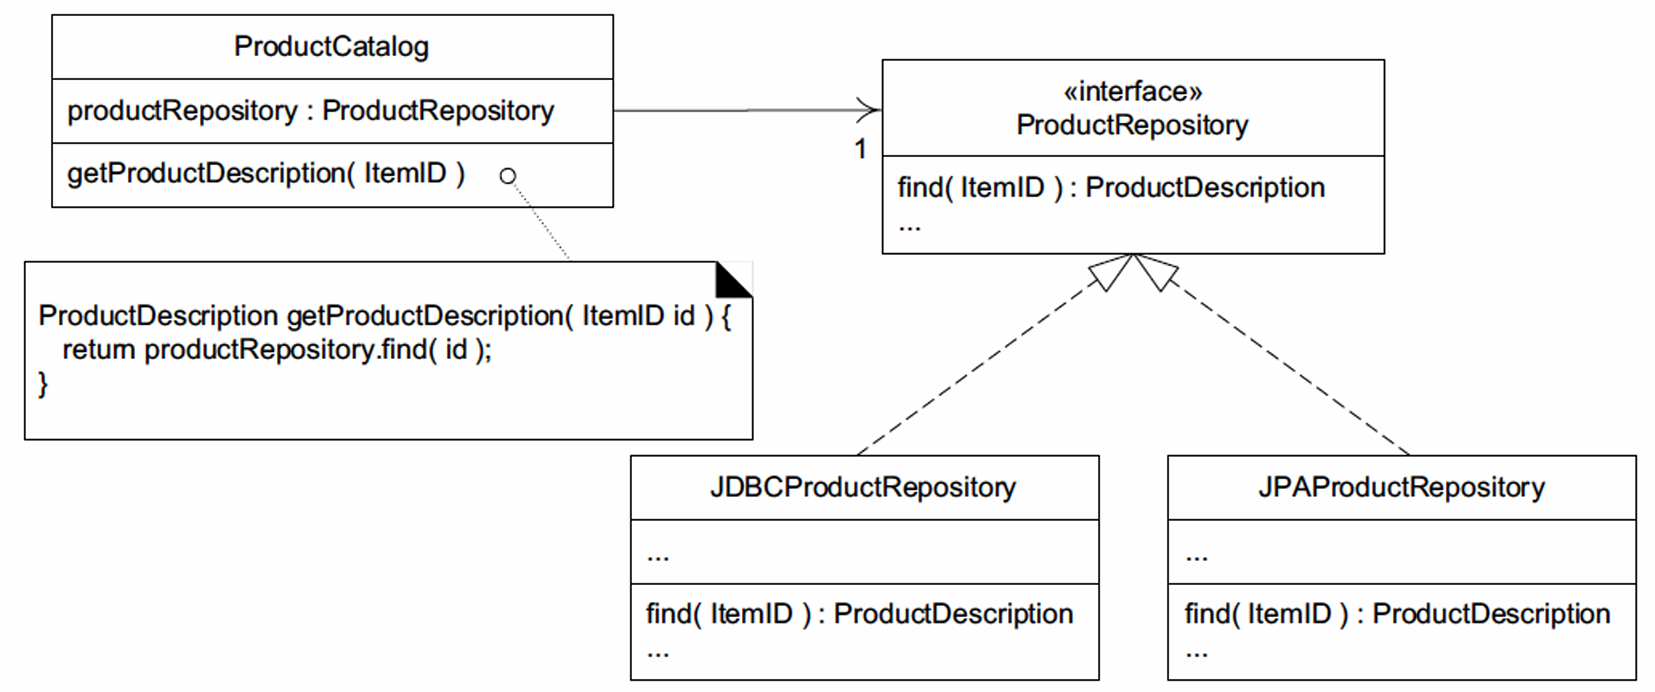
\includegraphics[scale=0.27]{Esercitazione - Design Patterns/repository_pattern.png}
    \end{center}

    In questo esempio abbiamo 3 componenti:
    \begin{enumerate}
        \item \textbf{ProductRepository} è l'interfaccia che funge da repository dei prodotti, viene usata per
        accedere alle informazioni di ciascun prodotto. tramite il metodo \textbf{find()}.
        \item \textbf{JDBCProductRepository} e \textbf{JPAProductRepository} sono delle\\ repository
        contenenti le informazioni.
        \item \textbf{ProductCatalog} è una classe che tramite l'\textit{ItemID} può ottenere la descrizione della
        repository corrispondente.
    \end{enumerate}
    \newpage
}

\mysubsectionformatted{Failover}
\myparagraph{
    Prima di parlare di failover, bisogna definire 3 termini apparentemente uguali:
    \begin{tcolorbox}[colback=green!5!white, colframe=green!75!black]
        \textbf{Fault (Guasto/Difetto):} L'origine o la causa di un comportamento sbagliato
    \end{tcolorbox}

    \begin{tcolorbox}[colback=purple!5!white, colframe=purple!75!black]
        \textbf{Error (Errore):} La manifestazione di un difetto nel sistema
    \end{tcolorbox}

    \begin{tcolorbox}[colback=yellow!5!white, colframe=yellow!75!black]
        \textbf{Failure (Fallimento):} La mancata erogazione di un servizio causata da un errore
    \end{tcolorbox}
    
    \begin{tcolorbox}[colback=blue!5!white, colframe=blue!75!black]
        Per \textbf{Failover} si intende un meccanismo usato per garantire la continuità di un servizio in caso di
        un eventuale guasto o interruzione del sistema. Questo meccanismo agisce in maniera trasparente all'utente,
        simulando le operazioni del sistema principale.
    \end{tcolorbox}
    \vspace{0.1cm}
    \noindent L'obiettivo di un sistema è quello di garantire affidabilità, permettendo il \\ripristino in seguito a guasti esterni.
    La soluzione consiste nel:
    \begin{enumerate}
        \item \textbf{Rendere trasparente la locazione fisica dei dati}
        \item \textbf{Rendere il failover da remoto a locale}
        \item \textbf{Replicare parzialmente i servizi locali}
    \end{enumerate}

    \noindent Nel dettaglio, la soluzione consiste nell'usare un \textbf{Proxy} (fornito da una \\ \textit{ServicesFactory} di tipo Factory)
    in grado di gestire in maniera trasparente e sicura al client eventuali guasti, mascherando la locazione e la disponibilità dei servizi.
    Nel caso in cui un servizio dovesse essere non disponibile, il proxy effettua un failover verso un servizio secondario, senza che il client debba fare nulla.
    \\
    Altro obiettivo del Proxy è far si che realizzi delle implementazioni locali dei servizi remoti che hanno problemi, in modo
    che abbiano un comportamento semplificato e vincolato.
    \\
    Nel pratico, decidiamo di creare una cache locale di oggetti di tipo \\ \textit{ProductDescription}. In questo modo, avremo un aumento
    delle performance e dell'affidabilità.

    \newpage

    \mysubsubsectionformatted{Accesso alla cache locale}

    \begin{wrapfigure}{l}{0.5\textwidth}
        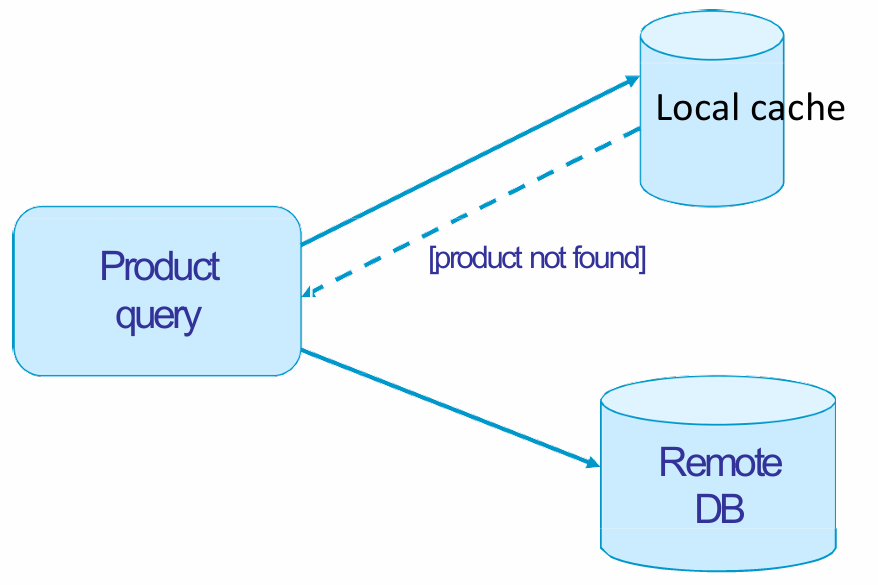
\includegraphics[scale=0.27]{Esercitazione - Design Patterns/Failover - Cache Locale.png}
    \end{wrapfigure}

    \hbadness=2000
    L'accesso alla cache locale avviene tramite il \textit{ServicesFactory}, questo ritorna un adapter a un servizio di 
    informazioni relativo ai prodotti in locale. L'adapter sarebbe l'entità che andrà a implementare le responsabilità del 
    servizio in locale, questo servizio sarà inizializzato con un riferimento verso un secondo adapter, ma quest'ultimo è 
    relativo al corrispondente servizio ma remoto.
    
    In sintesi, nel primo adapter abbiamo le responsabilità del servizio \textbf{locale}, il secondo adapter è relativo al corrispondente servizio
    locale ma in \textbf{remoto}. Se il servizio locale trova il prodotto nella cache (locale), allora lo ritorna, altrimenti inoltra la richiessta all'adapter
    del servizio remoto.
    
    Esistono due tipologie di cache:
    \begin{enumerate}
        \item Cache che mantengono in memoria una collezione di grandezza limitata ma dinamica (es. il \textit{ProductCatalog} che ha in memoria oggetti di tipo \textit{ProductDescription})
        \item Cache che mantengono in memoria una collezione più ampia di elementi su supporti persistenti (es. hard disk), questo implica che, se il sistema dovesse
        malfunzionare, la cache rimane persistente.
    \end{enumerate}

    \noindent \coloredtext[red]{Cosa succede se l'accesso alla cache locale non dà risultato e l'accesso al servizio esterno fallisce?}
    Si verificherà un \textbf{fallimento}, quindi bisogna gestirlo.
    \\
    Una soluzione comune sarebbe quella di \textbf{lanciare un'eccezione}, utile se l'errore si verifica a livello hardware. L'eccezione non deve essere percepita a 
    livello di presentazione (l'utente non deve vedere l'eccezione).
    \\
    Il pattern a cui si fa ricorso è il Design Pattern \coloredtext[blue]{\textbf{Convert Exceptions}} (descritto dopo il pattern Proxy).
    \newpage
}

\mysubsectionformatted{Design Pattern Proxy}
\myparagraph{

\begin{tcolorbox}[colback=blue!5!white, colframe=blue!75!black]
    Il pattern permette l'accesso a quegli oggetti che non sono direttamente\\ accessibili
    o non si desidera fornire l'accesso diretto. Viene creato un oggetto proxy che implementa
    la stessa interfaccia dell'oggetto ed è responsabile del controllo o del miglioramento dell'accesso
    a questo oggetto.
\end{tcolorbox}
\vspace{0.1cm}
    
\begin{center}
    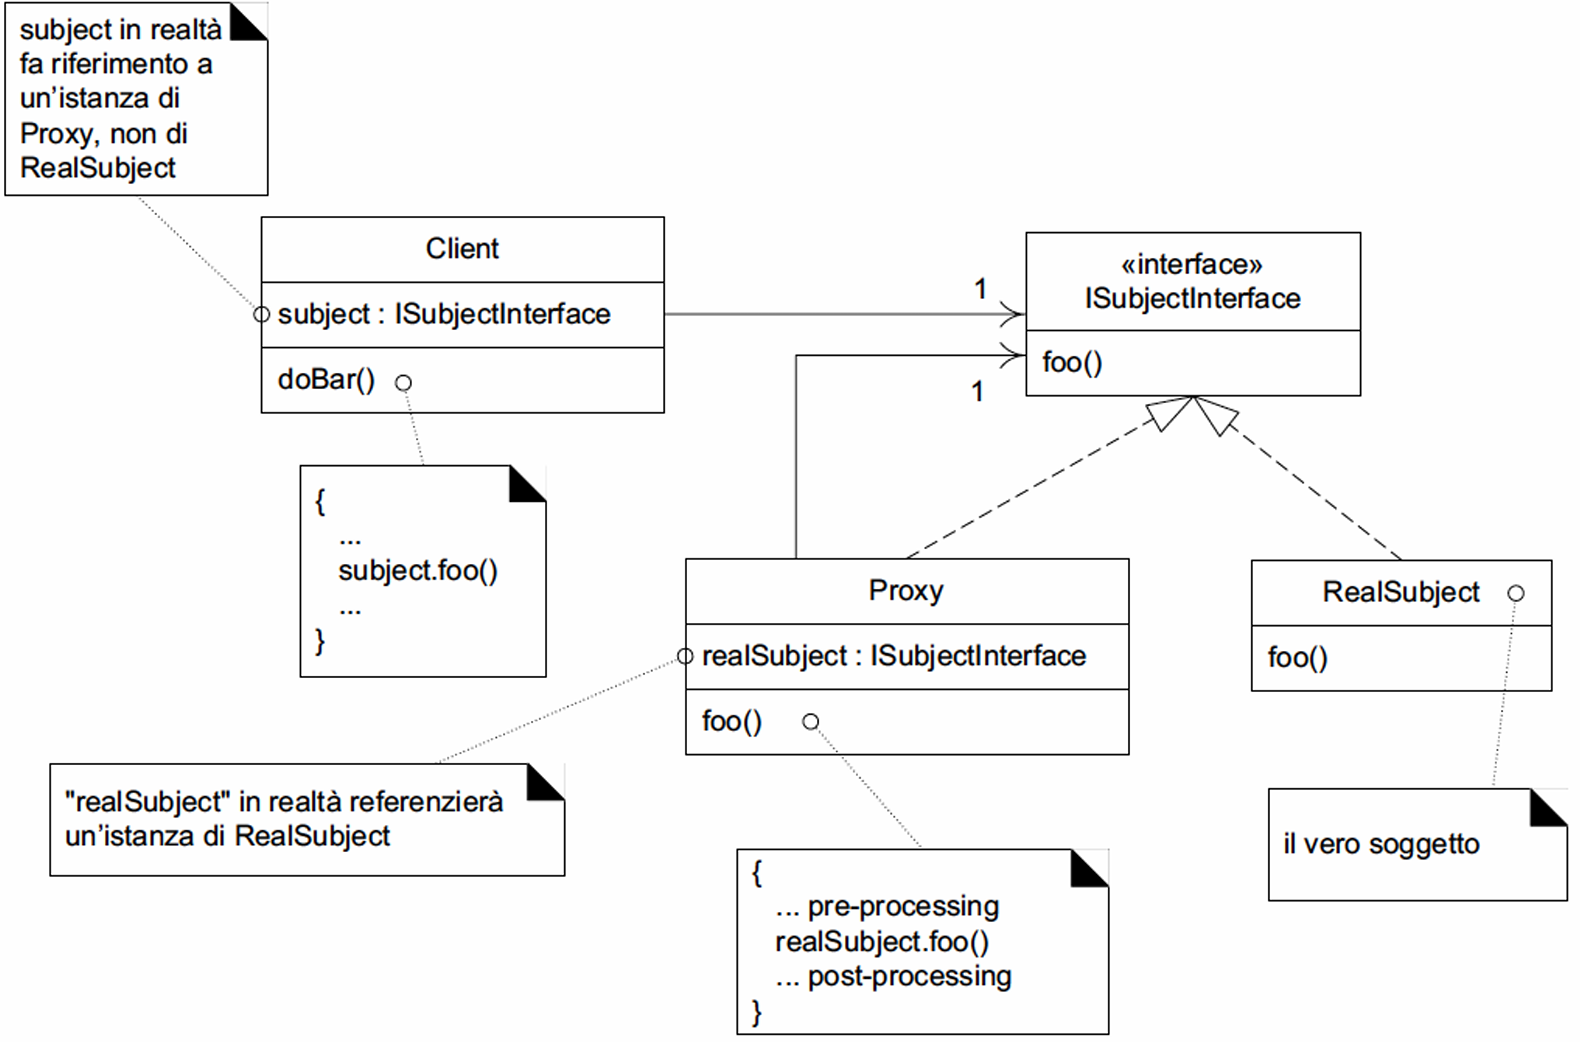
\includegraphics[scale=0.25]{Esercitazione - Design Patterns/proxy_pattern.png}
\end{center}
I componenti del pattern sono:
\begin{enumerate}
    \item \textbf{SubjectInterface} definisce un'interfaccia comune per l'oggetto reale\\ \textbf{RealSubject}
    e il \textbf{Proxy}, permettendo di usarli in modo alternabile.
    \item \textbf{RealSubject} è l'oggetto reale, contiene l'implementazione concreta della logica principale.
    \item \textbf{Proxy} è la classe che implementa la \textbf{SubjectInterface} e controlla l'accesso all'oggetto
    reale, implementando logica extra, contiene un riferimento al \textbf{RealSubject}.
\end{enumerate}
Esistono due strategie di gestione della cache:
\begin{enumerate}
    \item \textbf{Inizializzazione lazy}: la cache viene riempita lentamente man mano che vengono inseriti gli oggetti.
    \item \textbf{Inizializzazione greedy}: la cache viene caricata all'inizio.
\end{enumerate}

\newpage

\mysubsubsectionformatted{Ultime considerazioni sul Proxy}
\begin{enumerate}
    \item Il Proxy è un oggetto esterno che nasconde un oggetto interno.
    \item Il client non sa che sta facendo riferimento al Proxy, ma crede di comunicare direttamente con il sistema interno.
    \item Il Proxy è utile nel caso sia necessaria una ridirezione dei messaggi. 
\end{enumerate}

\newpage
    
}

\mysubsectionformatted{Design Pattern Convert Exceptions}
\myparagraph{
    \begin{tcolorbox}[colback=blue!5!white, colframe=blue!75!black]
        Il pattern permette di convertire un'eccezione di livello basso in un'eccezione più
        significativa a livello del sottosistema dove viene lanciata l'eccezione. L'eccezione
        di livello più alto avvolge quella di livello più basso e aggiunge informazioni per 
        renderla più significativa nel contesto del livello superiore. 
    \end{tcolorbox}

    \noindent Un consiglio è quello di rinominare l'eccezione in base al \textbf{perchè è stata \\lanciata, non come},
    in modo da rendere più semplificare al programmatore capire il problema.
 
    \begin{figure}[htbp]
        \centering
        \begin{minipage}{0.45\textwidth}
            \centering
            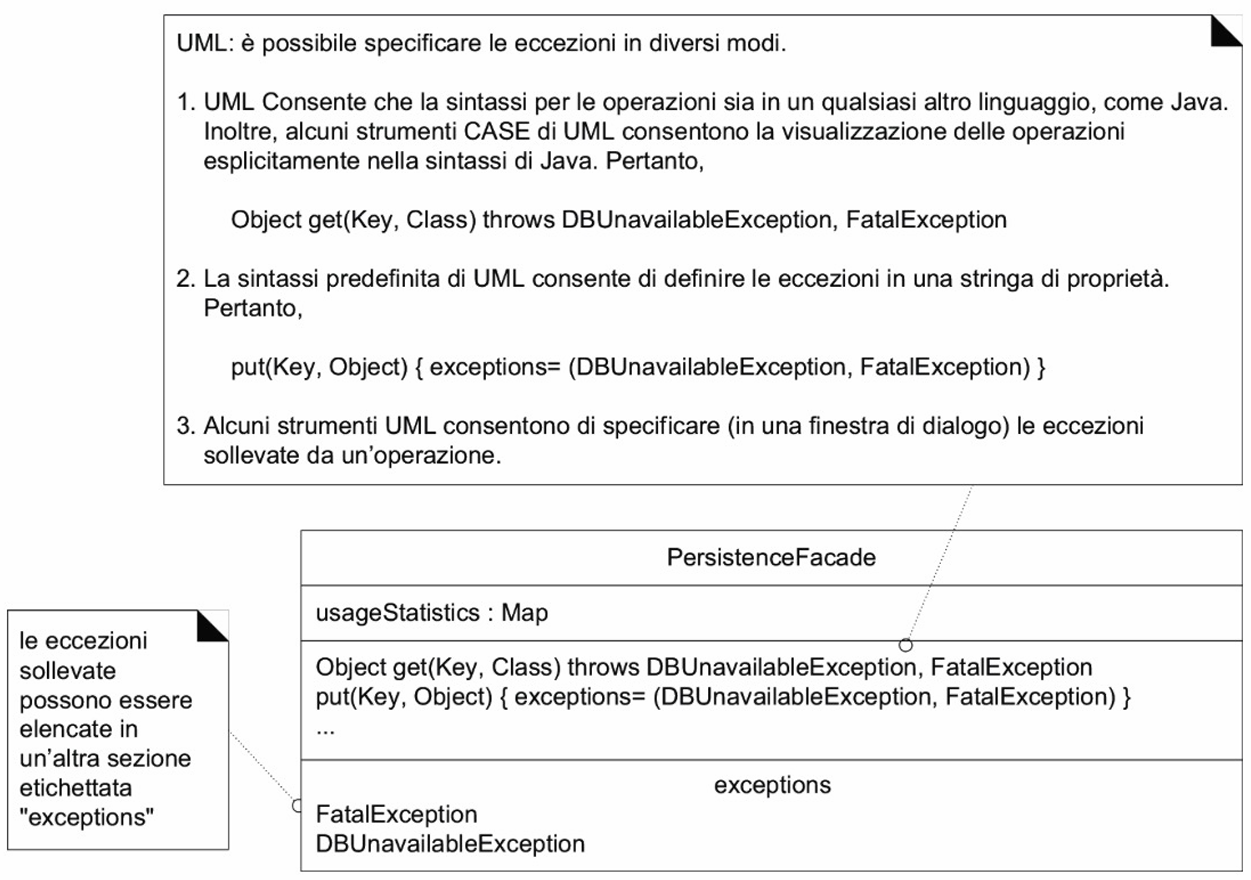
\includegraphics[width=\textwidth]{Esercitazione - Design Patterns/Eccezioni/UML_Eccezioni.png}
            \caption{Eccezioni in un diagramma delle classi}
            \label{fig:immagine1}
        \end{minipage}\hfill
        \begin{minipage}{0.45\textwidth}
            \centering
            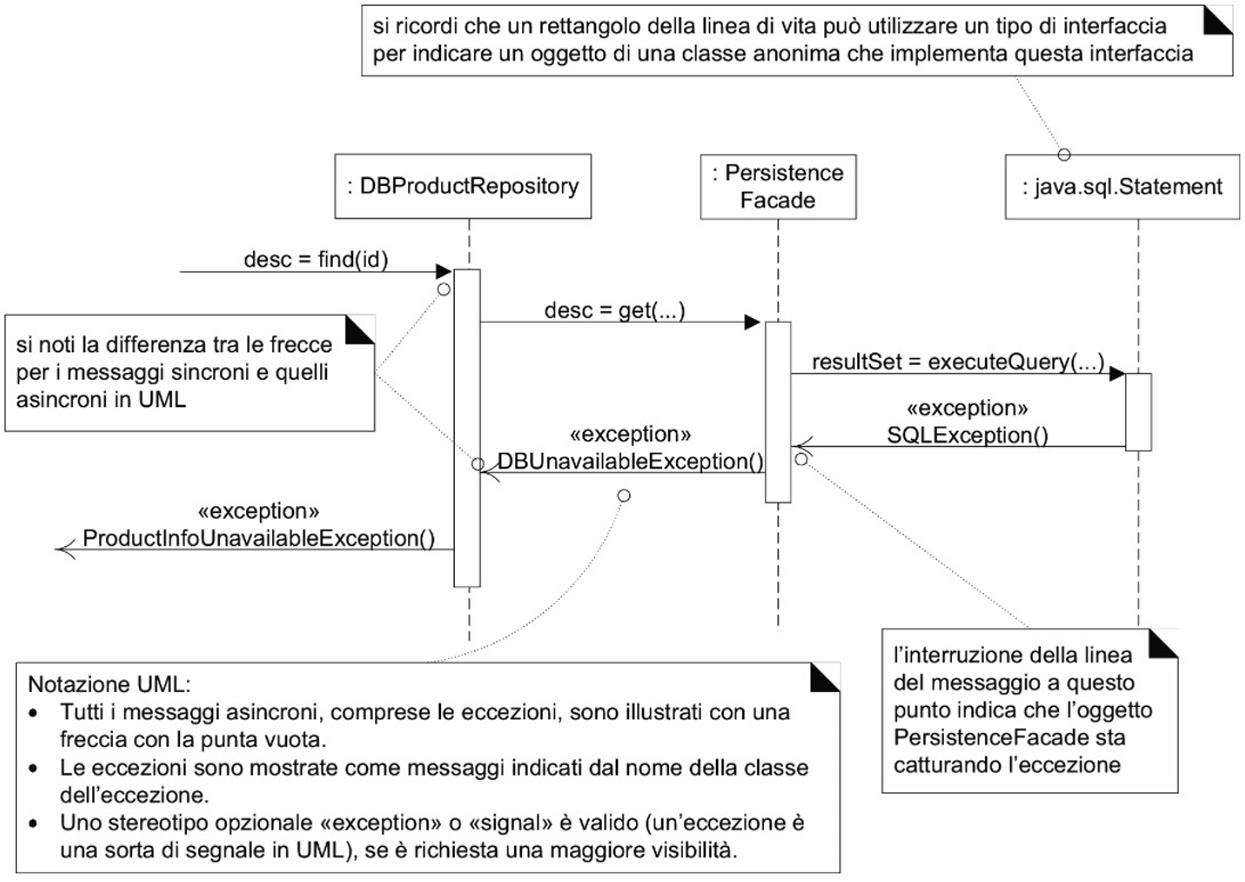
\includegraphics[width=\textwidth]{Esercitazione - Design Patterns/Eccezioni/Diagramma di Sequenza Eccezioni.png}
            \caption{Eccezioni in un diagramma di sequenza}
            \label{fig:immagine2}
        \end{minipage}
    \end{figure}
    \noindent Per gestire l'eccezione, può essere gestita tramite due pattern, il \coloredtext[blue]{\textbf{Centralized Error Logging}} e l'\coloredtext[blue]{\textbf{Error Dialog}}.
    \newpage
    }

\mysubsectionformatted{Design Pattern Centralized Error Logging}
\myparagraph{
    \begin{tcolorbox}[colback=blue!5!white, colframe=blue!75!black]
        Il pattern funge da oggetto centrale per il logging degli errori a cui si
        accede come un Singleton, e si riportano in esso tutte le eccezioni. In caso di
        sistema distribuito, ciascun Singleton locale collaborerà con un logger degli errori centrale.
    \end{tcolorbox}
    \vspace{0.1cm}   
}

\mysubsectionformatted{Design Pattern Error Dialog}
\myparagraph{
    \begin{tcolorbox}[colback=blue!5!white, colframe=blue!75!black]
        Il pattern permette di utilizzare un oggetto non appartenente all'interfaccia utente
        e accessibile attraverso un Singleton con lo scopo di comunicare gli errori agli utenti.
        Il pattern "avvolge" uno o più oggetti della UI (es. una finestra di testo), delegandogli
        la notifica dell'errore. Inoltre, ripoterà l'errore al logger centralizzato degli errori.
        Una \textit{Factory} ha il compito di creare l'oggetto UI appropriato in base ai parametri
        di sistema ricevuti, quindi in base all'errore.
    \end{tcolorbox}
}

\newpage

\mysubsectionformatted{Design Pattern Abstract Factory}
\myparagraph{
    \begin{tcolorbox}[colback=blue!5!white, colframe=blue!75!black]
        Il pattern permette di definire un'interfaccia astratta \textit{Factory} e
        altre classi \textbf{Factory} per ogni famiglia di elementi da creare.
        In questo modo, si possono creare delle famiglie di classi correlate tra loro
        che implementano un'interfaccia comune.
    \end{tcolorbox}

    \setcounter{figure}{0}
    \begin{figure}[h]
        \centering
        \caption{Esempio di Abstract Factory}
        \vspace{0.5cm}
        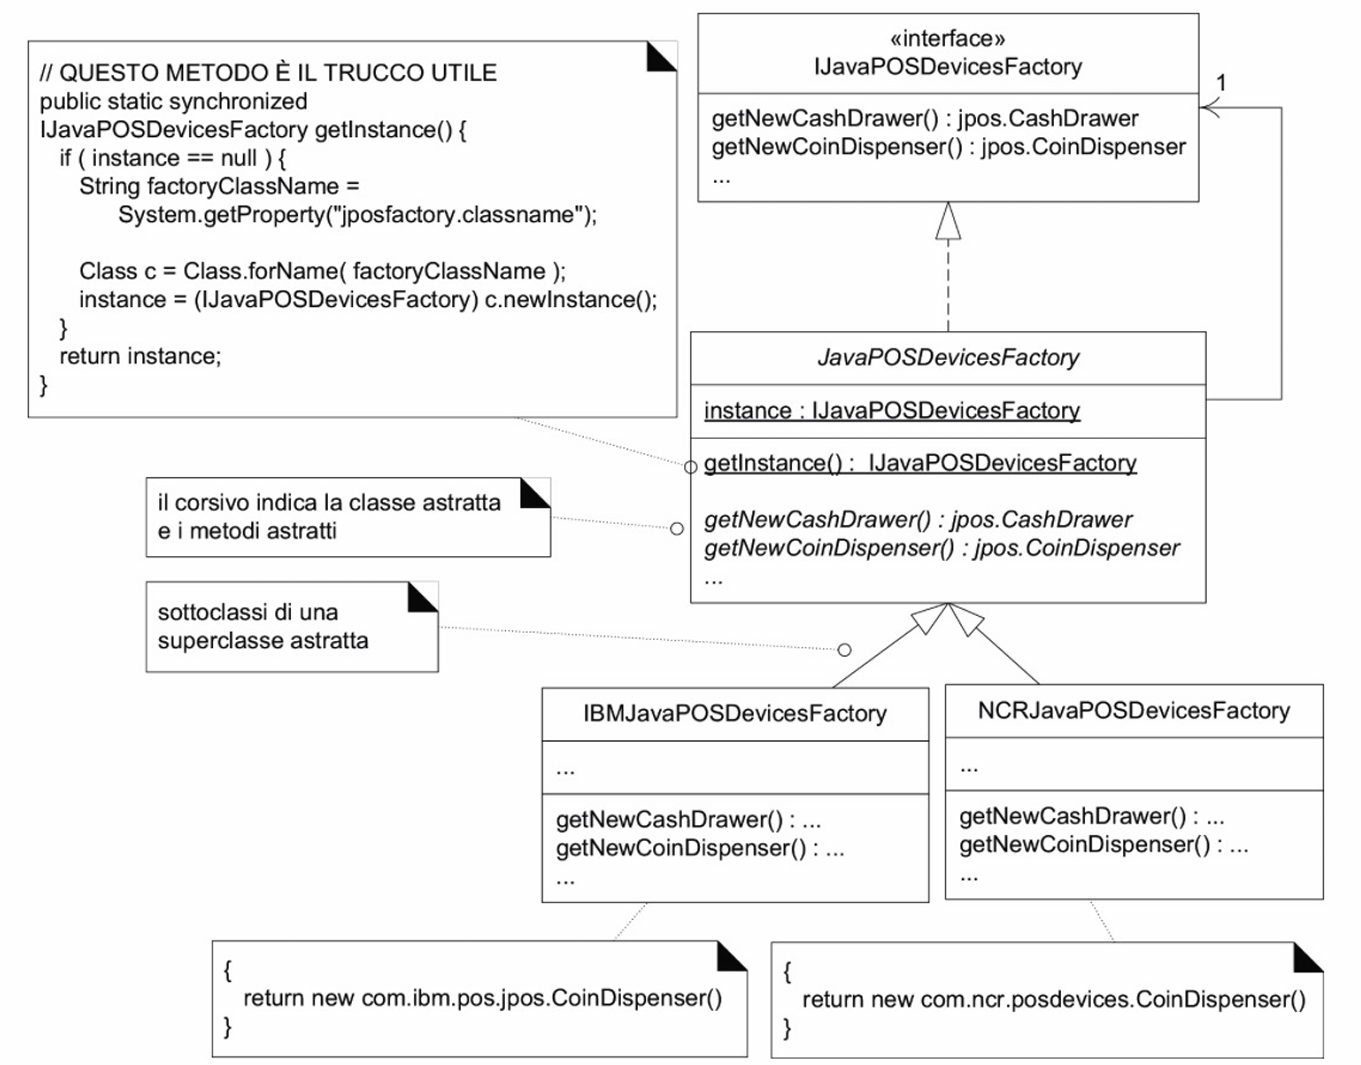
\includegraphics[scale=0.27]{Esercitazione - Design Patterns/Abstract Factory.png}
        \label{fig:pattern}
    \end{figure}

    Spesso, l'\textit{Abstract Factory} viene creata come \textbf{classe astratta}, non come \\interfaccia.\\
    La Factory legge dalle proprietà di sistema quale famiglia di oggetti creare, questo grazie all'aiuto
    del pattern \textbf{Singleton} (con il metodo \textit{getInstance()}).

    \newpage
    }


\mysubsectionformatted{Design Pattern Do It Myself}
\myparagraph{
    \begin{tcolorbox}[colback=blue!5!white, colframe=blue!75!black]
        Chiamato così da Peter Coad, il pattern ha l'obiettivo di applicare il \textbf{Polimorfismo},
        quindi far si che un oggetto software faccia quelle operazioni che normalmente
        verrebbero fatte all'oggetto reale di cui loro sono un'astrazione (loro intesi come gli oggetti software).  
    \end{tcolorbox}

    Detto in modo informale:
    \begin{itemize}
        \item Gli oggetti Quadrato creano se stessi.
        \item Gli oggetti Cerchio creano se stessi.
        \item Gli oggetti Text eseguono il controllo ortografico di se stessi.
    \end{itemize}

    \setcounter{figure}{0}
    \begin{figure}[h]
        \centering
        \caption{Uso del Polimorfismo con i mezzi di pagamento}
        \vspace{0.5cm}
        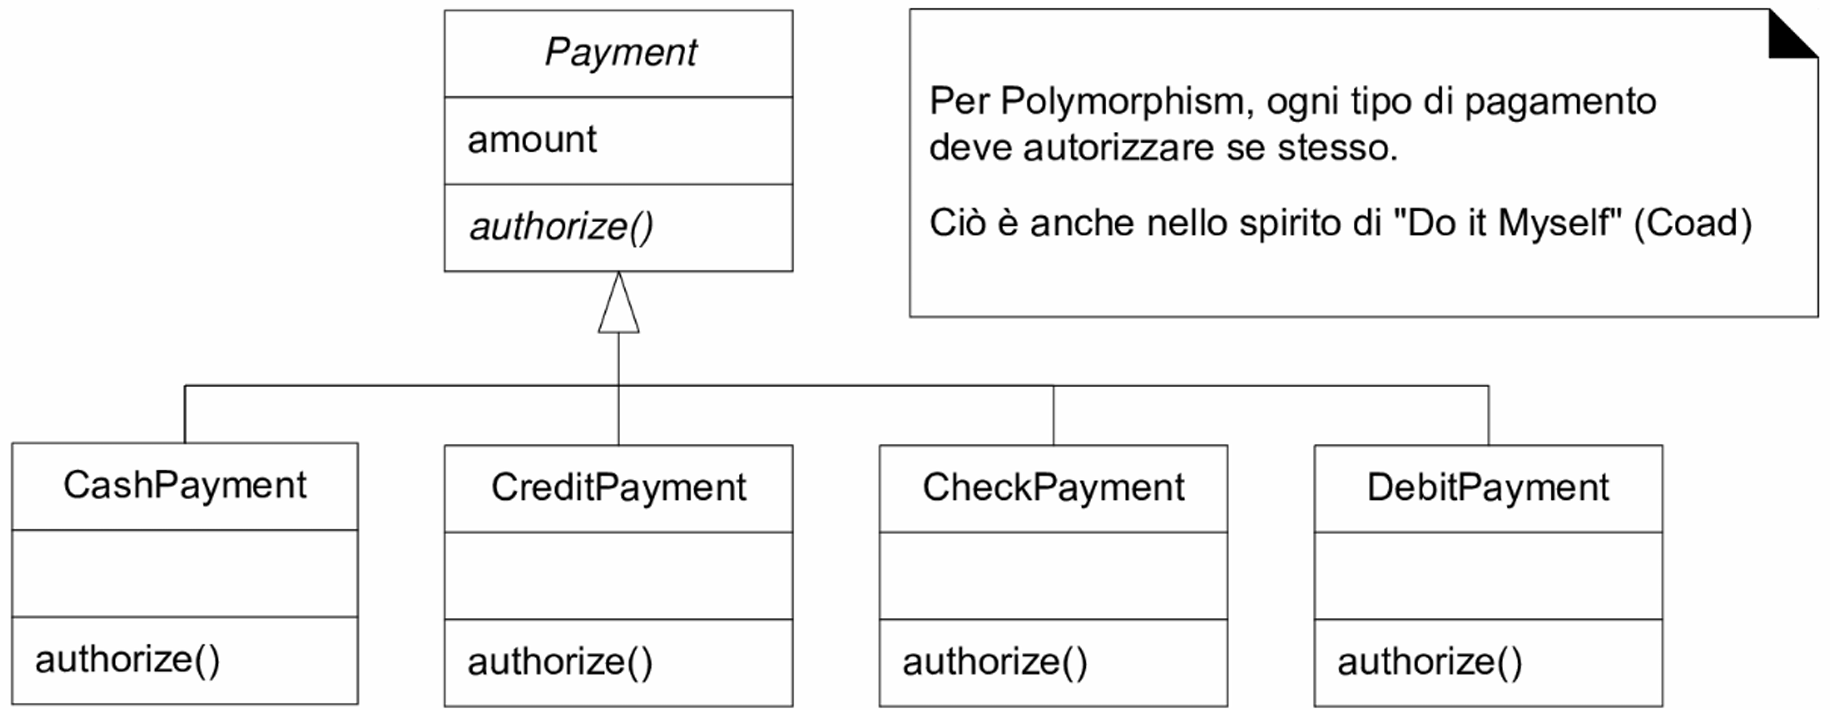
\includegraphics[scale=0.25]{Esercitazione - Design Patterns/Polymorphism.png}
        \label{fig:polymorphism}
    \end{figure}
}
\newpage

\mysubsectionformatted{Progettazione di Framework di persistenza dei dati}
\myparagraph{
    In questa esercitazione, si useranno 4 design pattern già visti per la progettazione
    di framework di persistenza dei dati:
    \begin{enumerate}
        \item Template Method
        \item State
        \item Command
        \item Proxy
    \end{enumerate}
    Quando parliamo di \textbf{Oggetti persistenti}, si intendono quegli oggetti che rimangono
    in memoria durante l'esecuzione del programma, quindi senza che vengano ripristinati alla fine
    dell'esecuzione.

    Solitamente, si fa ricorso ai \textit{database relazionali} che permettono di modellare un
    mapping tra la rappresentazione \textit{record oriented} del database e quella \textit{object-oriented}
    del sistema.

    Ecco alcune definizioni riguardo la persistenza:
    \begin{tcolorbox}[colback=blue!5!white, colframe=blue!75!black]
        Per \textbf{Framework di Persistenza} si intende un insieme di classi e interfacce riusabili, estendibili
        e \textit{general purpose}, che forniscono le funzionalità per la gestione degli oggetti persistenti.
    \end{tcolorbox}

    \begin{tcolorbox}[colback=green!5!white, colframe=green!75!black]
        Per \textbf{Servizio di Persistenza} si intente un sottosistema che fornisce le funzionalità per cooperare
        con il database e generalmente creato dal framework di persistenza.
    \end{tcolorbox}

    \begin{tcolorbox}[colback=red!5!white, colframe=red!75!black]
        Per \textbf{Oggetti Persistenti} si intendono quegli oggetti che necessitano di memorizzazione persistente.
    \end{tcolorbox}

    \mysubsubsectionformatted{Proprietà dei framework}
    \hbadness=10000
    \begin{enumerate}
        \item \`E un insieme coeso di interfacce e classi che collaborano tra loro per fornire servizi per la parte
        fondamentale e invariabile di un sottosistema logico.
        \item Contiene classi concrete e astratte che definiscono le interfacce a cui conformarsi e le interazioni tra
        gli oggetti.
        \item Di solito, richiede all'utente di definire delle sottoclassi di classi esistenti del framework per personalizzare
        ed estendere i servizi del framework.
        \item Ha delle classi astratte che possono contenere metodi astratti e concreti.
    \end{enumerate}

    \mysubsubsectionformatted{Servizio di persistenza}
    Un compito fondamentale del \textbf{Servizio di Persistenza} è quello di \textbf{effettuare il mapping fra
        la rappresentazione a oggetti e rappresentazione relazionale dei dati}, per farlo, compie due operazioni:
    \begin{enumerate}
        \item \textbf{Materializzazione}: traduzione di record in oggetti (caricamento in memoria).
        \item \textbf{Dematerializzazione}: traduzione di oggetti in record (memorizzazione nel DB).
    \end{enumerate}

    Per creare un servizio di persistenza, si deve realizzare un framework di persistenza che abbia le seguenti funzionalità:
    \begin{enumerate}
        \item Memorizzazione e recupero degli oggetti in e da un sistema di storage persistente.
        \item Fornire transazioni coerenti di \textbf{commit} e \textbf{rollback}.
        \item Deve essere estendibile per poter supportare diversi meccanismi e formati di memorizzazione (es. XML).
    \end{enumerate}

    I \textbf{punti chiave} per progettare un framework di persistenza sono:
    \begin{enumerate}
        \item Mapping.
        \item Indetificazione univoca degli oggetti.
        \item Materializzazione e Dematerializzazione degli oggetti (mediante pattern \textit{Template}).
        \item Gestione dello stato degli oggetti persistenti (mediante pattern \textit{State}).
        \item Modellazione delle operazioni relative a una transazione quali commit e rollback (mediante pattern \textit{Command}).
        \item Lazy materialization (mediante pattern \textit{Proxy}).
        \item Aumento delle performance con l'uso della cache.
    \end{enumerate}

    \newpage
    \mysubsubsectionformatted{Mapping}
    Il mapping risponde alla domanda \textit{"Come facciamo a far corrispondere un oggetto a un record in un DB relazionale?"}

    \subsubsection{Design Pattern Representing Objects as Tables}
    Un pattern utile allo scopo è il \coloredtext[blue]{\textbf{Representing Objects as Tables}}.
    \myparagraph{
    \begin{tcolorbox}[colback=blue!5!white, colframe=blue!75!black]
        Il pattern permette di definire una tabella per ciascuna classe di oggetti persistenti
        dentro un DB relazionale. Gli attributi degli oggetti corrisponderanno alle colonne della tabella e
        conterranno oggetti di tipo primitivo.
    \end{tcolorbox}
}

    \mysubsubsectionformatted{Identificazione univoca di oggetti}
    Questo punto chiave permette di non ripetere la materializzazione di oggetti molteplici volte, col rischio di creare oggetti
    duplicati.

    \subsubsection{Design Pattern Object Identifier}
    Il pattern utile allo scopo è l'\coloredtext[blue]{\textbf{Object Identifier}}.
    \myparagraph{
    \begin{tcolorbox}[colback=blue!5!white, colframe=blue!75!black]
        Il pattern permette di assegnare a ogni record di tabella e a ogni oggetto un
        valore alfanumerico chiamato Object ID che consente l'immediata identificazione
        di ogni istanza.
    \end{tcolorbox}

    \begin{center}
        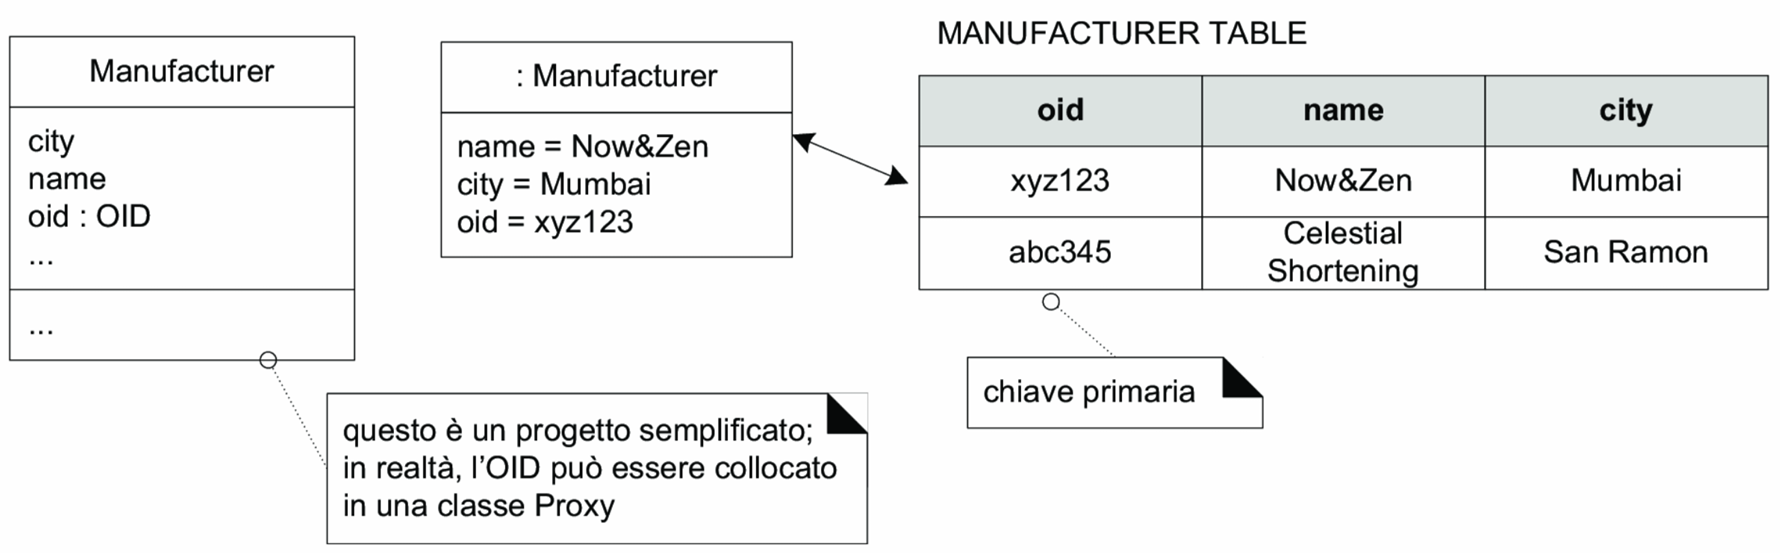
\includegraphics[scale=0.25]{Esercitazione - Design Patterns/Object Identifier.png}
    \end{center}
}

    \newpage
    \mysubsubsectionformatted{Accesso a un Servizio di Persistenza}
    Un pattern utile a fornire un unico punto di accesso è il \textbf{Facade}.
    \subsubsection{Design Pattern Facade}
    \myparagraph{
    \begin{tcolorbox}[colback=blue!5!white, colframe=blue!75!black]
        Il pattern fornisce un'interfaccia unificata ai servizi forniti di un certo sottosistema.
        La Facade delega le richieste provenienti dai client verso gli oggetti del sottosistema che nasconde. 
        Il suo intento è quello di rendere più semplice l'uso di un sottosistema.
    \end{tcolorbox}

    \vspace{0.1cm}
    \begin{center}
        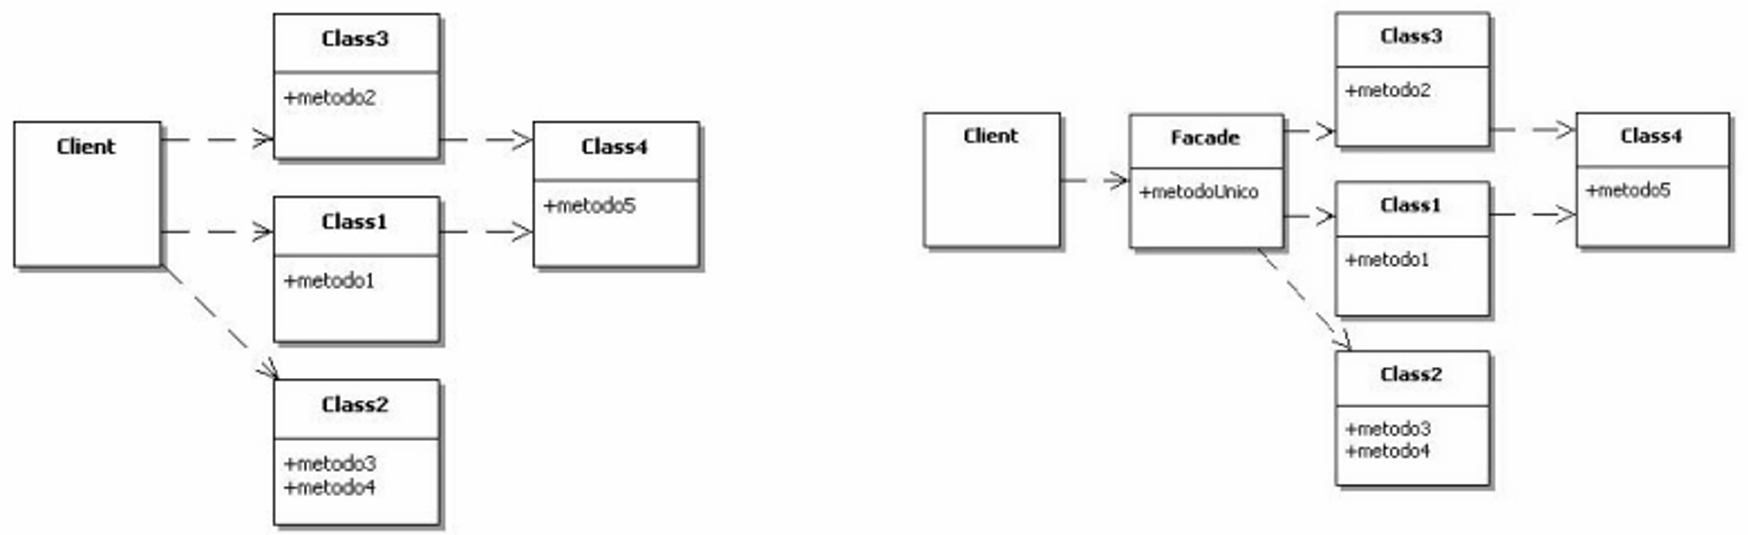
\includegraphics[scale=0.25]{Esercitazione - Design Patterns/Facade.png}
    \end{center}
    I partecipanti del pattern sono:
    \begin{enumerate}
        \item \textbf{Facade}: Conosce le classi responsabili per una richiesta e delega le richieste dei client
        agli oggetti appropriati del sottosistema.
        \item \textbf{Classi del sottosistema}: Implementano le funzionalità del sottosistema e gestiscono il lavoro
        assegnato dal Facade, questo però senza aver alcun riferimento di quest'ultima.
    \end{enumerate}

    Bisogna fare alcune considerazioni riguardo questo pattern:
    \begin{enumerate}
        \item Diminuisce l'accoppiamento tra client e sottosistema.
        \item Nasconde al client le componenti del sottosistema.
        \item Il client può comunque usare direttamente le classi del sottosistema.
    \end{enumerate}
    Si può anche rendere il Facade una classe astratta con sottoclassi concrete per diminuire ulteriormente
    l'accoppiamento. I client possono comunicare con il sottosistema mediante l'interfaccia della classe astratta Facade.

    \mysubsubsectionformatted{Facade vs Adapter}
    \begin{enumerate}
        \item Entrambi sono dei wrapper.
        \item Entrambi si basano su un'interfaccia, però:
        \item \begin{enumerate}
            \item Facade lo semplifica.
            \item Adapter lo converte.
        \end{enumerate}
    \end{enumerate}
}

    \mysubsubsectionformatted{Materializzazione e Dematerializzazione}
    In questa sezione vedremo \textbf{chi si occupa della Materializzazione e \\l'archiviazione degli oggetti}.

    Esistono due tipi di \textbf{Mapping}:
    \begin{enumerate}
        \item \textbf{Direct Mapping}: una classe che rappresenta un oggetto persistente \\definisce al suo interno il codice
              per il suo salvataggio nel DB (il codice è generato in automatico).
        \item \textbf{Indirect Mapping}: esistono classi apposite volte al recupero e al salvataggio dei dati in un DB.
    \end{enumerate}

    Questi due tipi di mappature si possono rappresentare mediante due pattern: \coloredtext[blue]{\textbf{Active Record}} per il Direct e \coloredtext[blue]{\textbf{Database Mapper}}
    per l'Indirect.

    \newpage
    \mysubsectionformatted{Active Record - Direct Mapping}
\myparagraph{
    \begin{tcolorbox}[colback=blue!5!white, colframe=blue!75!black]
        Il pattern architetturale permette di convertire ciascuna classe di dominio in tabella del DB.
        Combina i dati e il comportamento di un'entità in un'unica classe e inserisce la
        logica di accesso ai dati nell'oggetto di dominio, in modo che tutti sappiano come leggere e
        scrivere i dati da/al DB.
    \end{tcolorbox}
    
    \begin{center}
        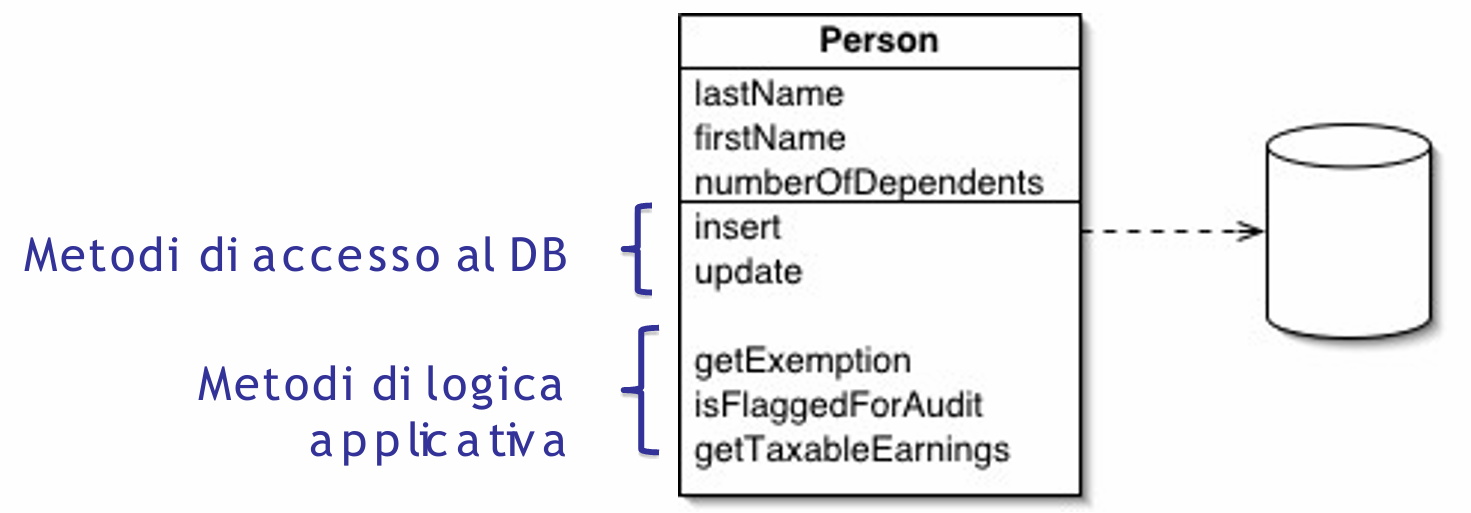
\includegraphics[scale=0.25]{Esercitazione - Design Patterns/Active Record.png}
    \end{center}

    Active Record fa uso di alcuni metodi e strutture dati:
    \begin{enumerate}
        \renewcommand{\labelenumii}{\arabic{enumi}.\arabic{enumii}}
        \item \textbf{Metodo load}: costruisce un'istanza partendo dai risultati generati da una query SQL.
        \item \textbf{Metodi finder} statici: incapsulano le query SQL e ritornano le istanze degli oggetti.
        \item \textbf{Costruttore classico}: costruisce nuove istanze da inserire successivamente nel DB.
        \item \textbf{Metodi di aggiornamento del DB}:
              \begin{enumerate}
                  \item \textbf{update}: aggiorna un record esistente con i valori degli attributi.
                  \item \textbf{insert}: aggiunge un record utilizzando i valori degli attributi.
                  \item \textbf{delete}: elimina il record corrispondente dell'oggetto corrente.
              \end{enumerate}
        \item \textbf{Metodi accessors}:
              \begin{enumerate}
                  \item I metodi \textbf{set} e \textbf{get} per accede ai campi.
                  \item Effettuano la conversione dei dati per memorizzare i valori degli attributi in un formato SQL-oriented.
                  \item Possono richiedere un'immediata sincronizzazione del DB.
              \end{enumerate}
        \item \textbf{Metodo di logica di business}
    \end{enumerate}
    \vspace{0.1cm}

    \resizebox{\columnwidth}{!}{%
        \begin{tabular}{l|l|}
            \hline
            \rowcolor[HTML]{32CB00}
            \multicolumn{1}{|c|}{\cellcolor[HTML]{32CB00}\textbf{Vantaggi}} & \multicolumn{1}{c|}{\cellcolor[HTML]{FE0000}\textbf{Svantaggi}}                                                                                     \\ \hline
            \multicolumn{1}{|l|}{Semplice da implementare e usare}          & \begin{tabular}[c]{@{}l@{}}L'accoppiamento fra la logica applicativa e il DB\\ rende difficile il refactoring dei due progetti\end{tabular}         \\ \hline
                                                                            & \begin{tabular}[c]{@{}l@{}}Si cerca di mantenere una corrispondenza stretta (o quasi)\\ fra lo schema del DB e l'entità del modello OO\end{tabular} \\ \cline{2-2}
        \end{tabular}%
    }
}
    \newpage
    \mysubsectionformatted{Database Mapper - Indirect Mapping}
\myparagraph{
    \begin{tcolorbox}[colback=blue!5!white, colframe=blue!75!black]
        Il framework (o pattern di progettazione) permette di definire una classe che si occupi della gestione dei processi
        di materializzazione da un DB, la dematerializzazione della memoria verso il DB e
        il caching degli oggetti con l'obiettivo di aumentare la performance del sistema.
    \end{tcolorbox}

    Il pattern definisce un DB Mapper per ogni classe di oggetti persistenti, possono esistere diversi
    tipi di Mapper a seconda dei meccanismi di memorizzazione.

    \begin{center}
        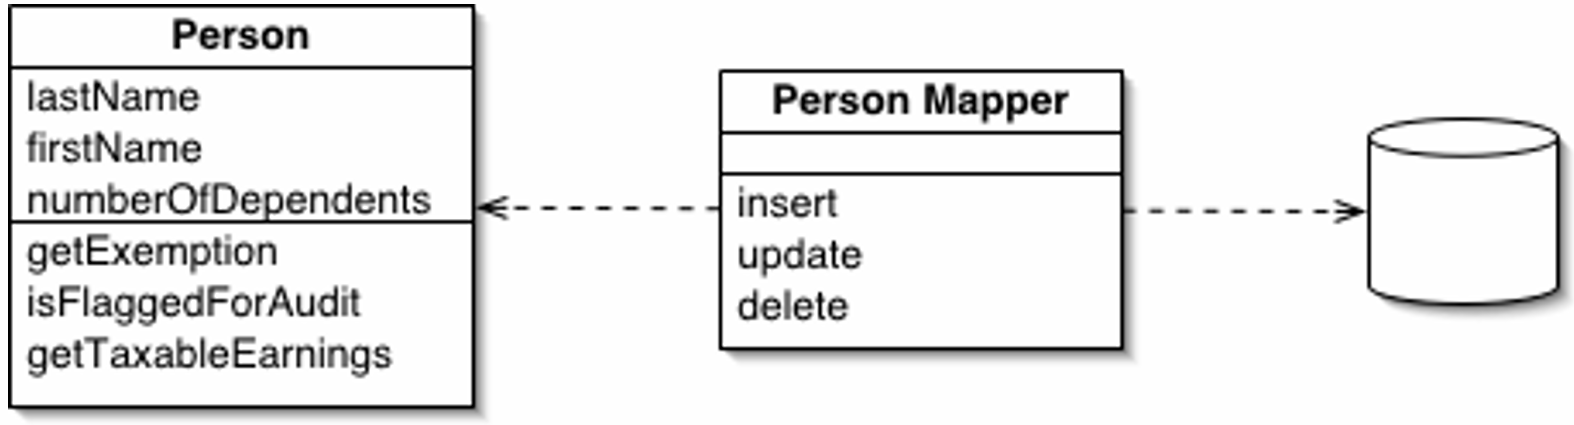
\includegraphics[scale=0.25]{Esercitazione - Design Patterns/Database Mapper.png}
    \end{center}

    \textbf{Person Mapper} è uno strato separato di componenti dedicati a trasferire i dati fra l'applicazione
    (\textbf{Person}) e il \textbf{Database}, trattando indipendentemente i due schemi (OO e ER). Infatti, la
    logica di business è inconsapevole dell'esistenza del Database.\\
    Generalmente, il pattern ne coinvolge di ulteriori per la gestione della sincronizzazione fra i due schemi
    (es. \textit{UnitOfWork} o \textit{IdentityMap}).\\
    Usiamo questo pattern per \textbf{gestire un mapping complesso fra DB e logica di business}.

    \begin{center}
        \resizebox{\columnwidth}{!}{%
            \begin{tabular}{ll}
                \hline
                \rowcolor[HTML]{32CB00}
                \multicolumn{1}{|c|}{\cellcolor[HTML]{32CB00}\textbf{Vantaggi}} & \multicolumn{1}{c|}{\cellcolor[HTML]{FE0000}\textbf{Svantaggi}} \\ \hline
                \multicolumn{1}{|l|}{Isola totalmente i due strati}             & \multicolumn{1}{l|}{Difficolta nell'implementazione}            \\ \hline
                                                                                &
            \end{tabular}%
        }
    \end{center}
    \newpage
}

    \mysubsectionformatted{Materializzazione in cache}
    Vogliamo mantenere all'interno della cache locale gli oggetti che sono stati materializzati in modo da:
    \begin{enumerate}
        \item Aumentare le prestazioni
        \item Supportare la gestione delle transazioni
    \end{enumerate}

    Il pattern utile allo scopo è il \coloredtext[blue]{\textbf{Cache Management}}
    \mysubsubsectionformatted{Design Pattern Cache Management}
    \myparagraph{
    \begin{tcolorbox}[colback=blue!5!white, colframe=blue!75!black]
        Il pattern estende il design pattern \textbf{Database Mapper}, facendo si che siano
        responsabili per la gestione della cache. Ogni Mapper può mantenere e gestire una propria
        cache privata. Il pattern verifica prima di tutto se gli oggetti sono in cache
        prima di recuperarli dal DB per evitare materializzazioni inutili.
    \end{tcolorbox}
}
    L'algoritmo di materializzazione, in pseudocodice, è strutturato in questo modo:
    \vspace{-0.1cm}
    \begin{algorithm}
        \caption{Gestione Cache}
        \begin{algorithmic}[1]
            \If{l'oggetto è in cache}
            \State ritorna l'oggetto
            \Else
            \State materializza l'oggetto dal database
            \State salva l'oggetto in cache
            \State ritorna l'oggetto
            \EndIf
        \end{algorithmic}
    \end{algorithm}
    \vspace{-0.1cm}

    Per progettare questa funzionalità, il pattern utile allo scopo è il \textbf{Template Method} (visto nella prima esercitazione).
    Il template method sarà il metodo \textbf{get} in una superclasse astratta. Ogni mapper specifico darà poi la sua implementazione
    di come ottenere i propri oggetti dal repository.

    \setcounter{figure}{0}
    \begin{figure}[H]
        \caption{Template Method per la materializzazione}
        \centering
        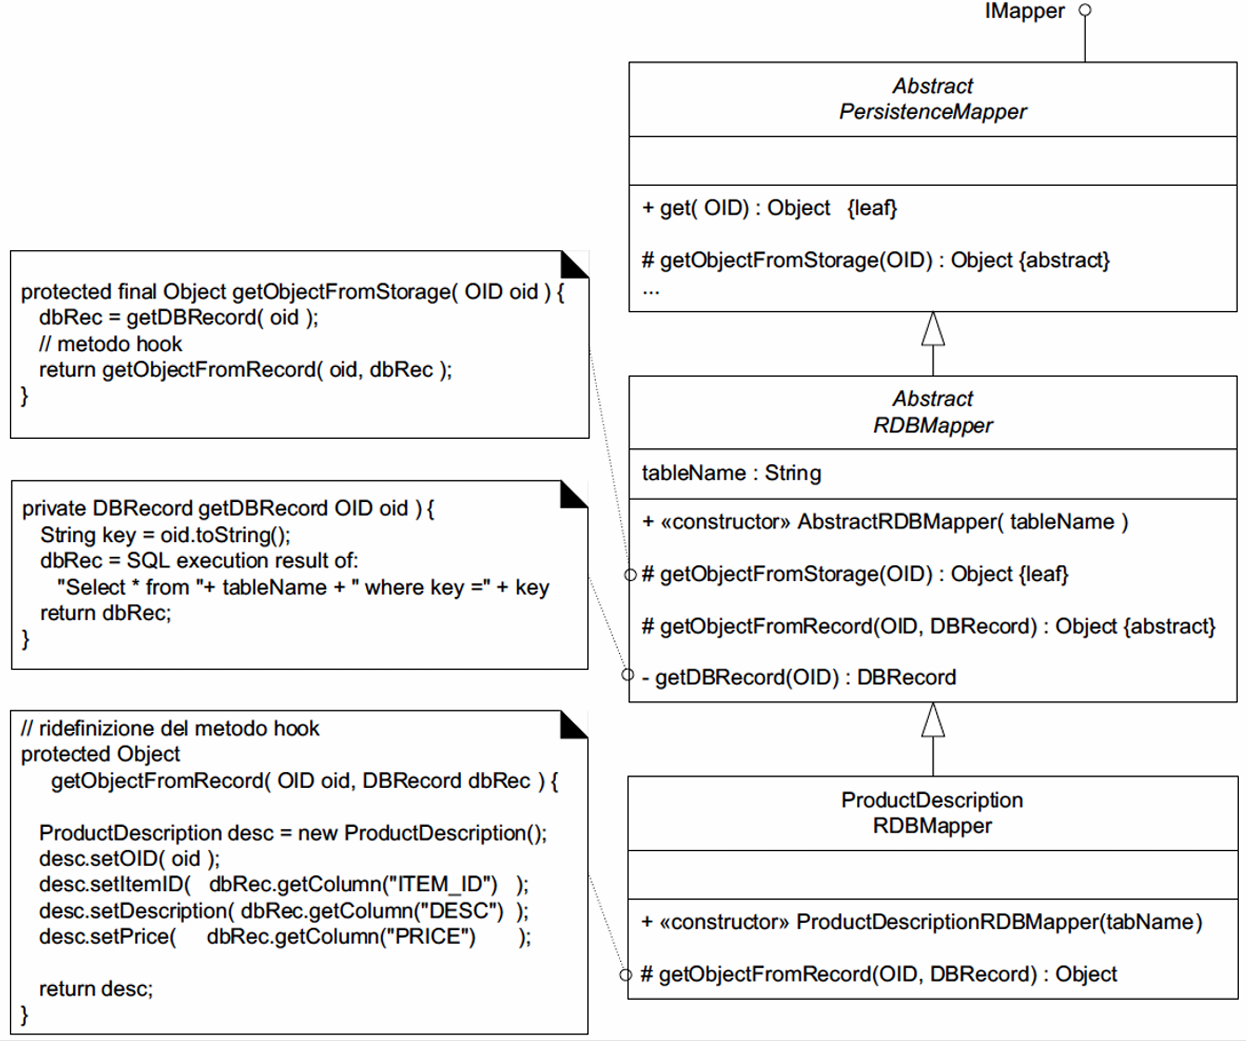
\includegraphics[scale=0.18]{Esercitazione - Design Patterns/Template Method Materializzazione.png}
    \end{figure}

    \newpage
    Fino ad'ora, le query SQL sono sempre state inserite dentro al codice dei metodi.

    \begin{center}
        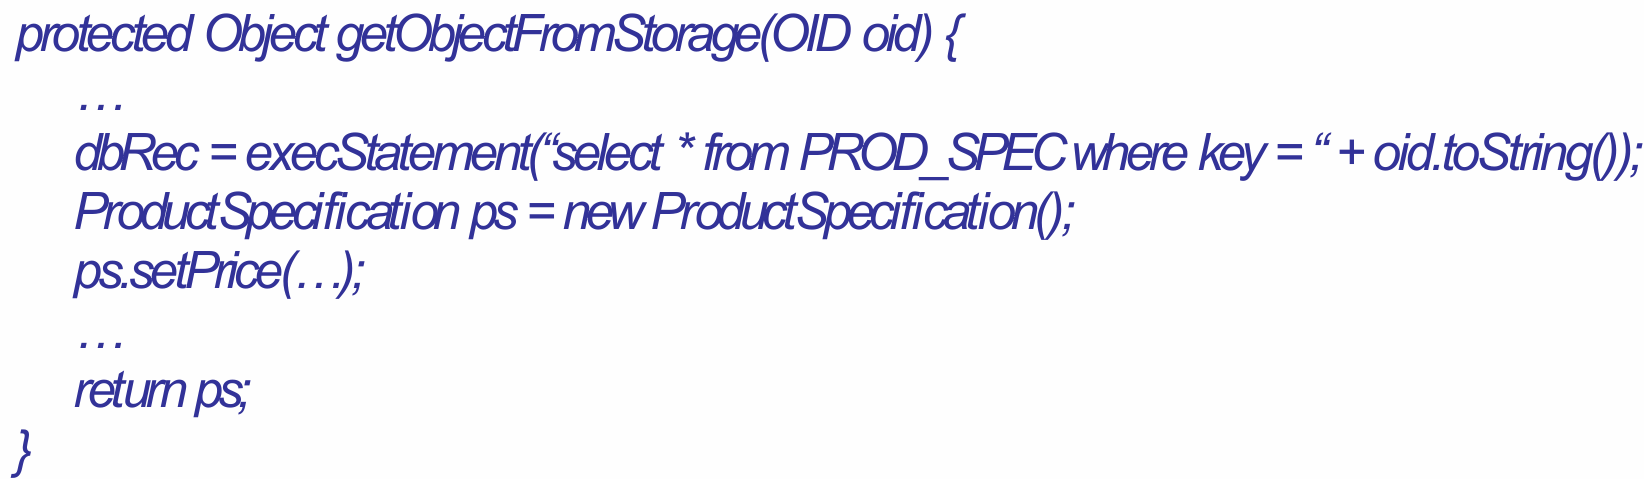
\includegraphics[scale=0.25]{Esercitazione - Design Patterns/Template Method SQL/Fase 1.png}
    \end{center}

    Per migliorare l'implementazione,
    si può mantenere una classe \textbf{Singleton} dove memorizzare tutte le query SQL necessarie (RDBOperations).

    \begin{center}
        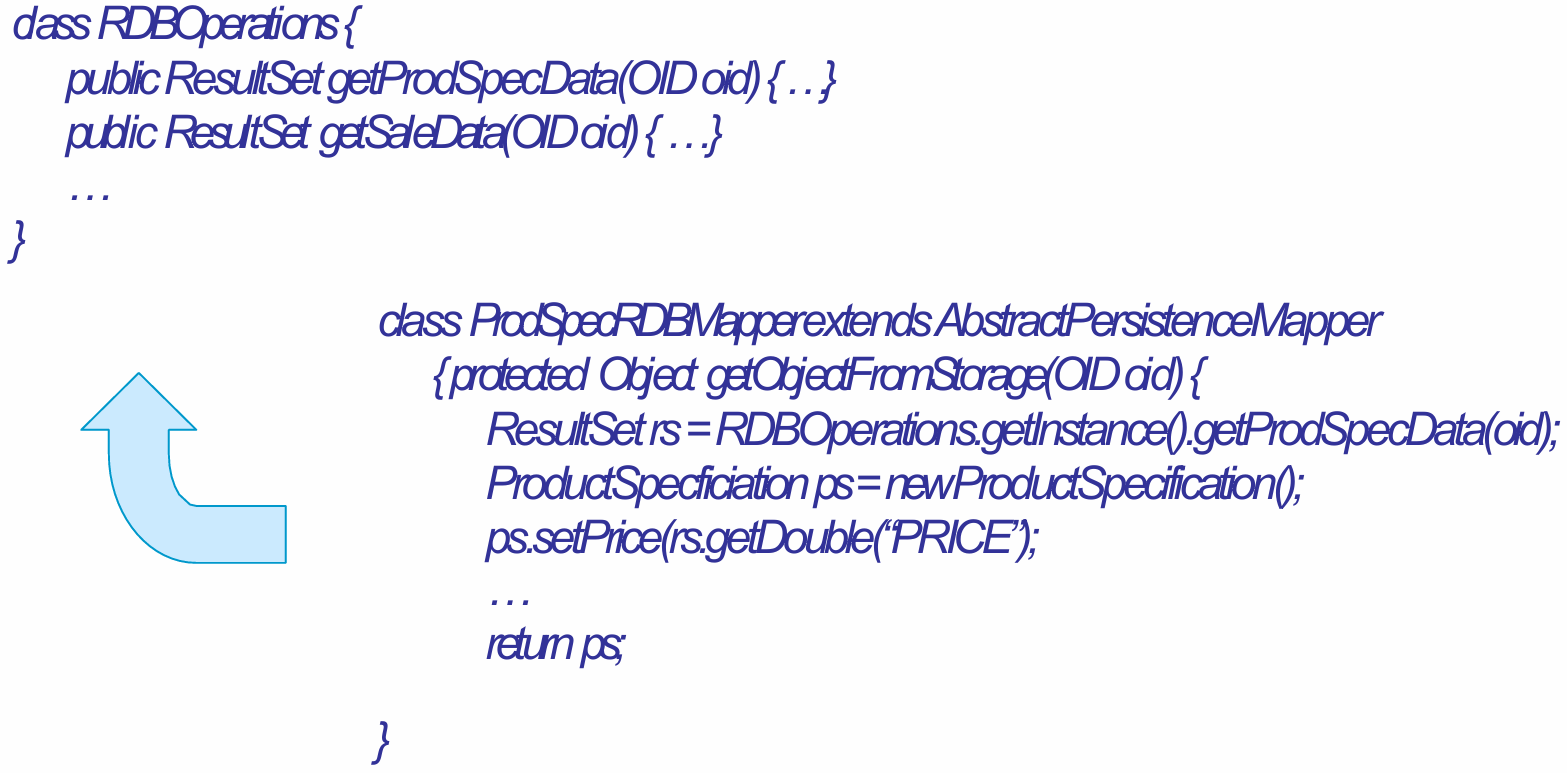
\includegraphics[scale=0.25]{Esercitazione - Design Patterns/Template Method SQL/Fase 2.png}
    \end{center}

    Risulta vantaggioso isolare le query in modo da rendere più facile la manutenzione migliorare la performance.
    \newpage
    }

\mysubsectionformatted{Transazioni e Stati transazionali}
\myparagraph{
    Una \textbf{Transazione} è un'unità di lavoro i cui compiti devono essere completati tutti con successo,
    oppure nessuno di essi deve essere completato. 

    Quando lavoriamo su oggetti persistenti (li inseriamo, cancelliamo o aggiorniamo), questi non vengono aggiornati
    subito nel database, bisogna quindi eseguire un'operazione di commit esplicita.
    Possiamo definire \textbf{3 luoghi} in cui possono trovarsi gli oggetti persistenti:
    \begin{enumerate}
        \item nell'applicazione
        \item nel database
        \item nella cache
    \end{enumerate} 

    Si possono anche definire gli \textbf{stati} associati agli oggetti persistenti:
    \begin{enumerate}
        \item \textbf{New}: appena creato e non ancora presente nel DB
        \item \textbf{Old}: recuperato dal DB (quindi creato in precedenza) 
        \item \textbf{Clean}: non modificato
        \item \textbf{Dirty}: modificato
        \item \textbf{Deleted}: cancellato
    \end{enumerate}

    \setcounter{figure}{0}

    \begin{figure}[h]
        \caption{Diagramma degli Stati}
        \centering
        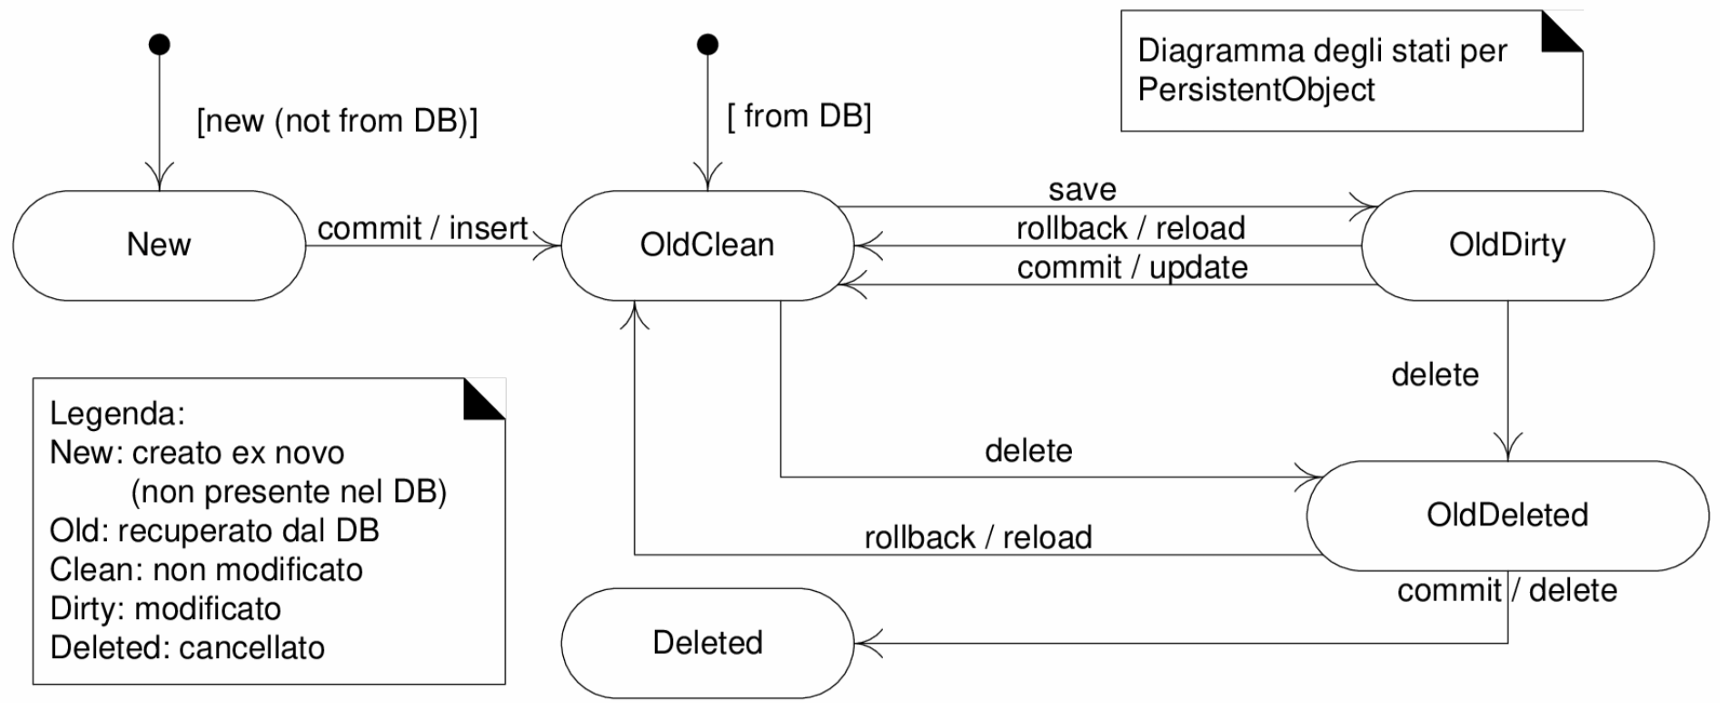
\includegraphics[scale=0.27]{Esercitazione - Design Patterns/Diagramma degli Stati.png}
    \end{figure}
    \textbf{Nota:} quando salviamo o cancelliamo un oggetto persistente, questo non viene immediatamente
    salvato/cancellato dal DB, ma vanno in uno stato appropriato (OldDirty o OldDeleted) in attesa di un eventuale rollback
    (annullo l'operazione) o commit (procedo con l'operazione).
    \newpage
    Il comportamento di \textbf{commit} e \textbf{rollback} sono molto simili tra loro (in termini di codice)

    \begin{center}
        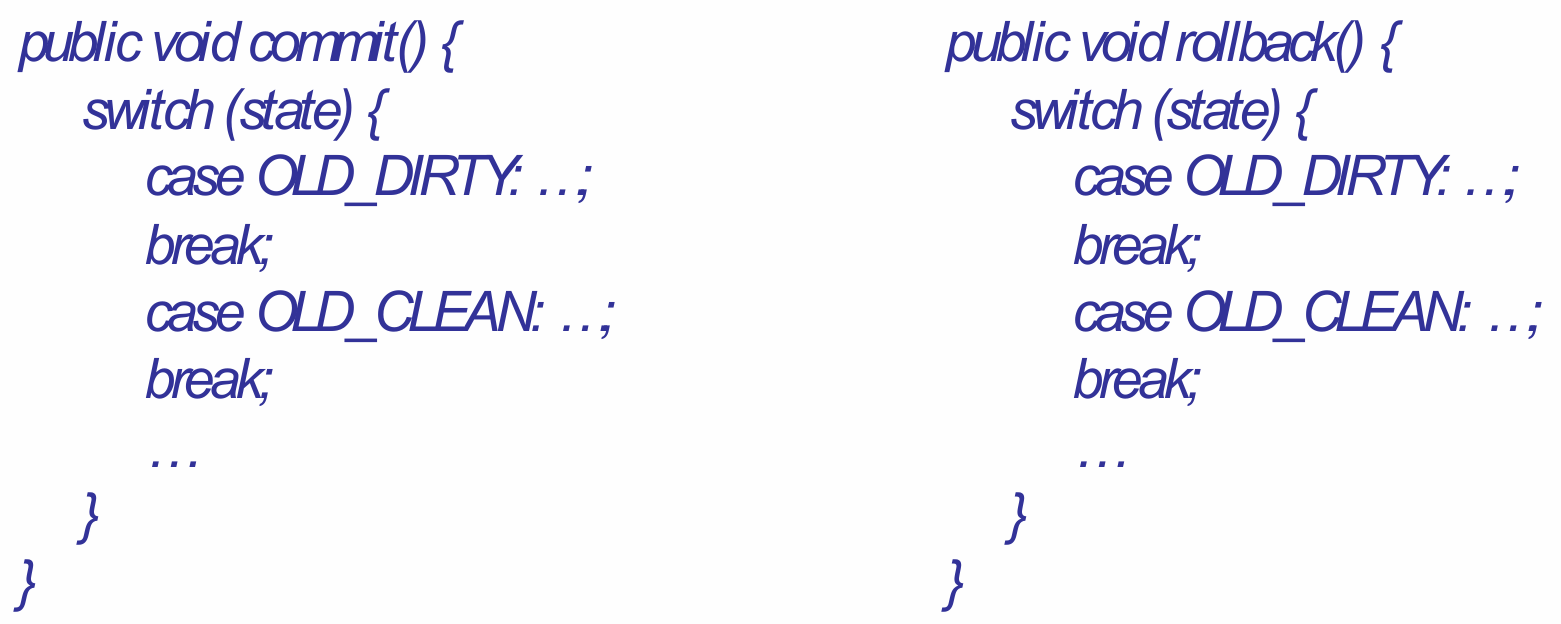
\includegraphics[scale=0.25]{Esercitazione - Design Patterns/Commit e Rollback.png}
    \end{center}
    Per evitare una ripetizione di codice, usiamo il pattern \textbf{State}:
    \begin{center}
        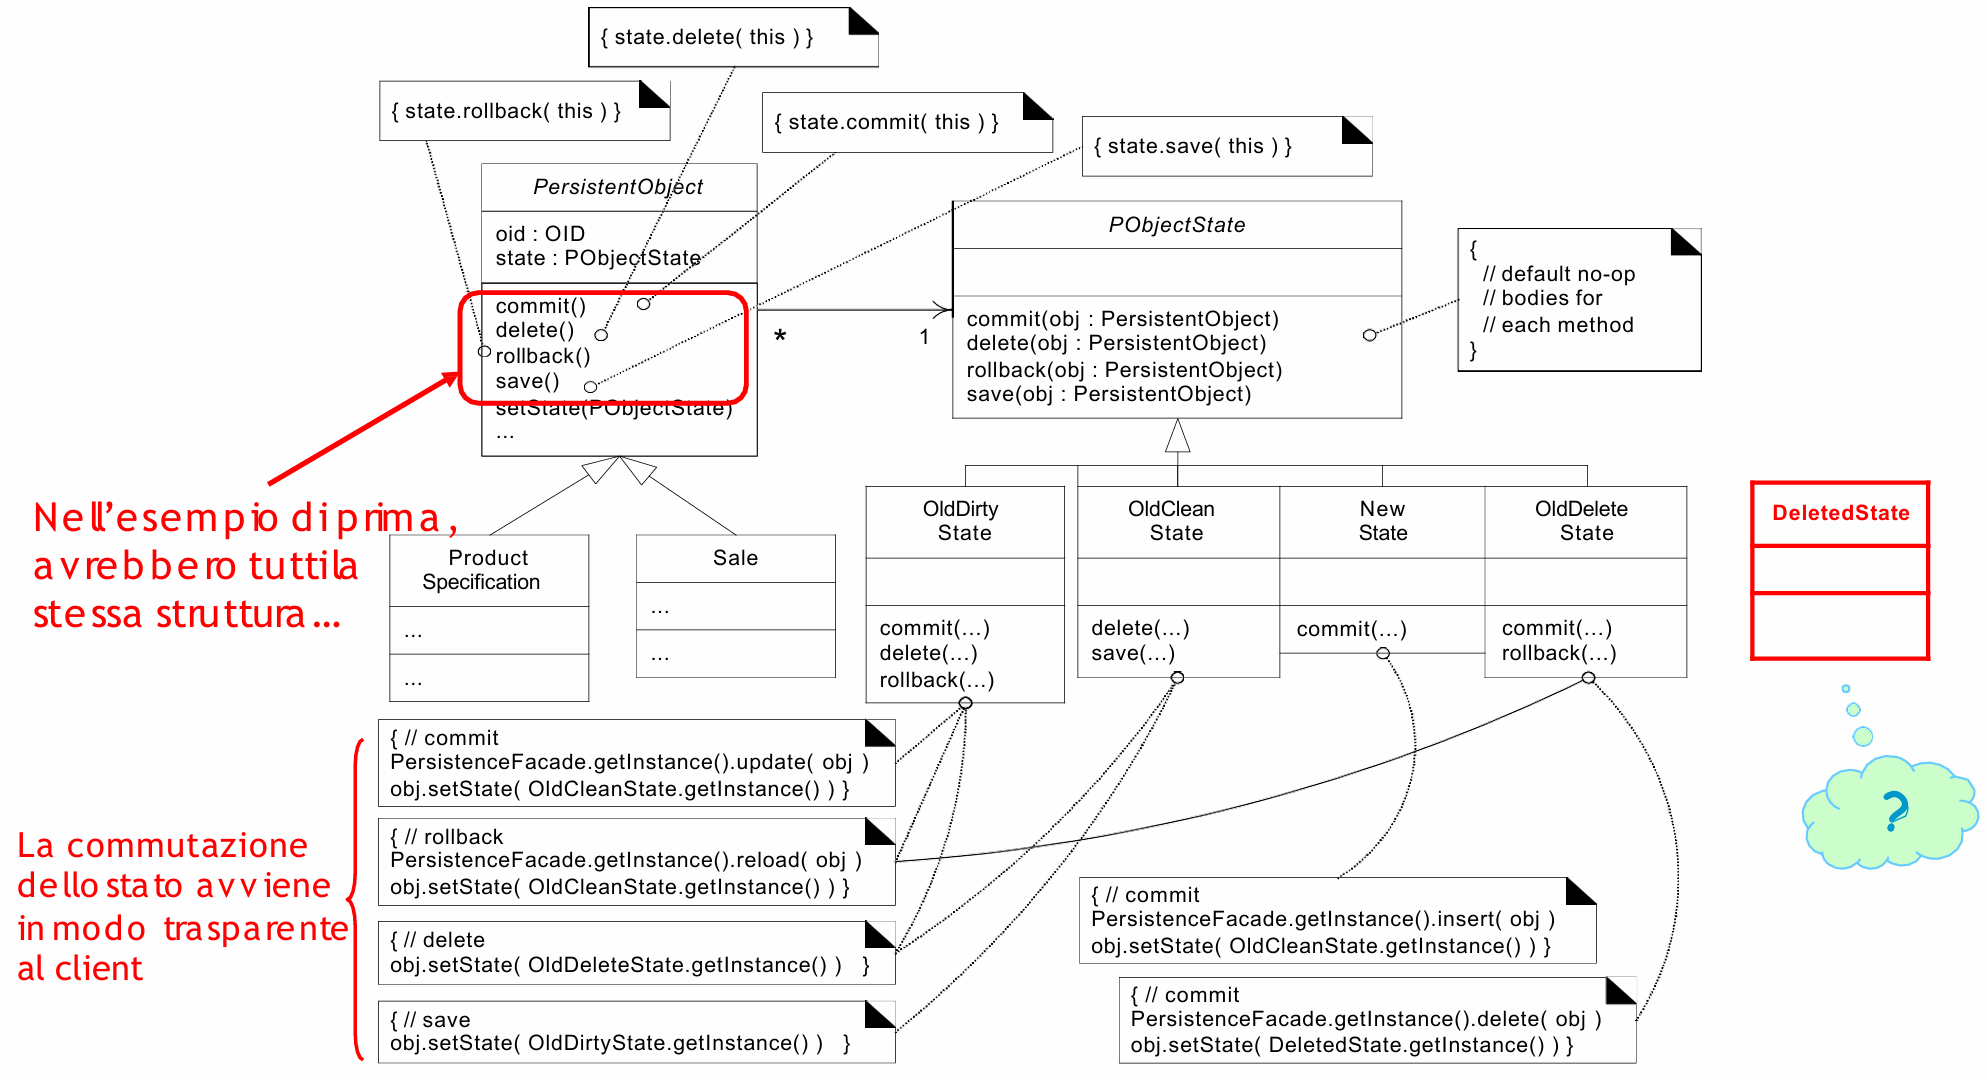
\includegraphics[scale=0.24]{Esercitazione - Design Patterns/State con Commit e Rollback.png}
    \end{center}
    Ricordando cosa fa lo State, crea delle classi che indicano gli stati, le classi implementano un'interfaccia
    comune. Questa interfaccia delega le operazioni all'oggetto \textbf{contesto} in base al suo stato corrente.

    Nell'esempio sopra il \textit{PersistentObject} rappresenta l'oggetto \textbf{Context}, mentre \textit{PObjectState}
    l'interfaccia \textbf{\textit{State}}. Per ogni stato concreto, definiamo le operazioni appropriate.
    \newpage
    \mysubsubsectionformatted{Modellazione delle operazioni di una transazione}
    Le transazioni, ovviamente, possono essere molteplici. In base all'ordine in cui vengono eseguite le operazioni all'interno
    di una transazione, si può influenzare la performance della transazione. Bisogna quindi trovare una soluzione, ovvero un modo
    per poter riordinare tutte le operazioni uguali prima di essere eseguiti. In questo ambito, interviene il pattern \textbf{Command}.
    
    Ricordando cosa fa Command, definisce per ciascun compito una classe che implementa un'interfaccia comune, a differenza di State che
    rappresentava uno stato, \textbf{nel Command ciascuna classe rappresenta un comando} e le azioni diventano oggetti.
    \begin{center}
        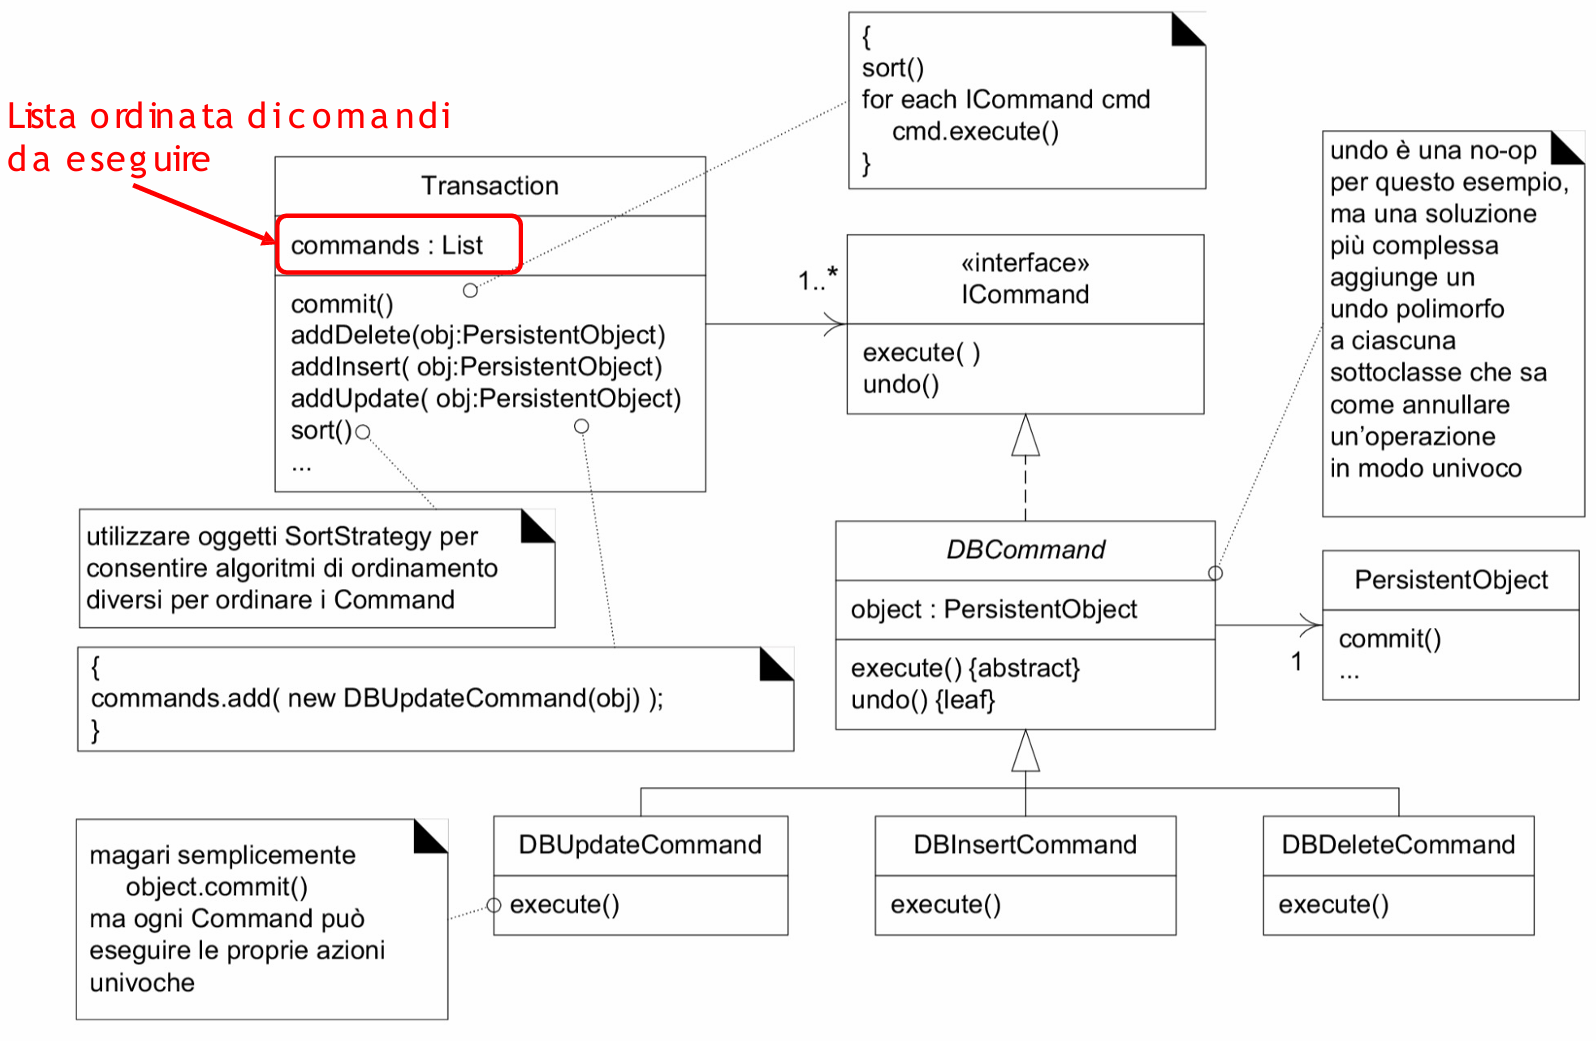
\includegraphics[scale=0.24]{Esercitazione - Design Patterns/Command con Commit e Rollback.png}
    \end{center}
    Nell'esempio, la classe Transaction è l'\textbf{invoker}, ovvero la classe che richiede all'interfaccia \textit{\textbf{ICommand}} le
    operazioni da eseguire. L'interfaccia riceve le operazioni e la classe DBCommand (la \textbf{ConcreteCommand}) incapsula le operazioni, per
    poi farle eseguire dal \textbf{Receiver}, ovvero la PersistentObject.
    \newpage
    \mysubsubsectionformatted{Lazy materialization con l'uso di Proxy}
    Ricordando la definizione di materializzazione, si tratta della traduzione di un record di un DB a un oggetto.

    A volte si vuole evitare il processo di materializzazione, per questioni di performance e a meno che non sia strettamente necessario. Si può
    risolvere questo problema tramite un processo di materializzazione "ritardata", ovvero la \textit{Lazy Materialization}.

    Il pattern utile allo scopo è il \coloredtext[blue]{\textbf{Virtual Proxy}}.
    \mysubsubsectionformatted{Design Pattern Virtual Proxy}
    \myparagraph{
    \begin{tcolorbox}[colback=blue!5!white, colframe=blue!75!black]
        Il Virtual Proxy è un Proxy per l'oggetto "reale", questo proxy virtuale
        materializza l'oggetto solo la prima volta a cui gli si fa riferimento,
        rappresentandoli come oggetti leggeri che fungono da sostituto all'oggetto
        reale (che possono essere più pesanti).
    \end{tcolorbox}

    In sostanza, il Virtual Proxy funge da sostituto dell'oggetto reale, ma in un formato
    più leggero. Sarà questo sostituto a gestire l'accesso all'oggetto reale e a caricarlo
    in memoria solo quando è strettamente necessario, in modo da evitare materializzazioni
    inutili.

    \begin{wrapfigure}{r}{0.55\textwidth}
        \begin{center}
          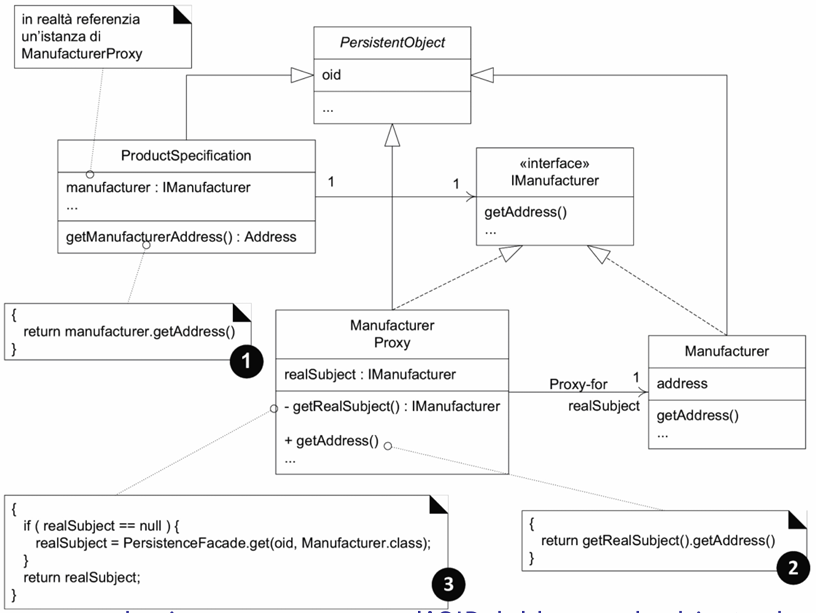
\includegraphics[width=0.55\textwidth]{Esercitazione - Design Patterns/Virtual Proxy.png}
        \end{center}
      \end{wrapfigure}
    
    \hbadness=2000
    Nell'esempio, Manufacturer è il nostro oggetto reale, \textbf{Manufacturer Proxy} è il suo \textbf{Virtual Proxy}, quindi
    un suo sostituto che ne gestisce l'accesso e stabilisce se caricarlo in memoria o meno. L'interfaccia comune \textit{IManufacturer}
    permette al client di interagire con il Virtual Proxy senza sapere che si tratta di un suo sostituto.

    Bisogna fare una considerazione, dato che parliamo di materializzazione ovviamente è coinvolto anche il pattern \textbf{DatabaseMapper},
    che in questo esempio è rappresentato dalla classe \textbf{ProductSpecification}, infatti questa crea un'istanza di \textit{IManufacturer},
    con lo scopo di decidere quali oggetti materializzare subito e a quali invece può ritardare questo processo. Si parla quindi di
    \textbf{Eager} e \textbf{Lazy Materialization}.

    \newpage
}
    \newpage
    \mysubsubsectionformatted{Eager vs Lazy Materialization}
\begin{center}
    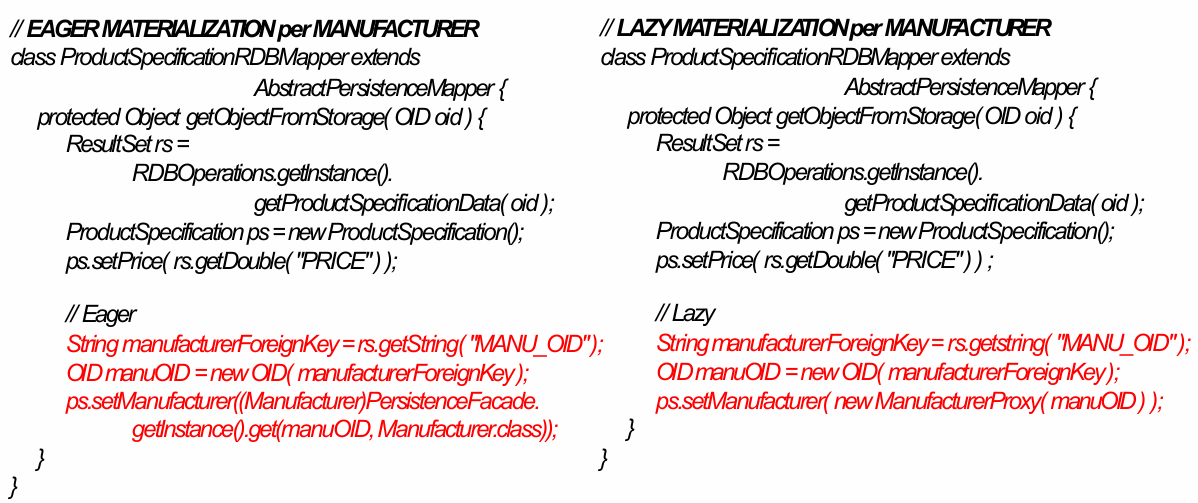
\includegraphics[scale=0.4]{Esercitazione - Design Patterns/Eager vs Lazy Materialization.png}
\end{center}

La differenza tra i due approcci sta nel caricamento in memoria del record in oggetto. Nel primo caso, avviene immediatamente
non appena i dati richiesti sono necessari, nel secondo caso il caricamento viene ritardato fino a quando l'oggetto non è
strettamente necessario.

Guardando il codice, entrambi gli approcci iniziano col prelevare la chiave\\ esterna del manifacturer, per poi creare un'ID da
associare all'oggetto (che verrà caricato in memoria) di quella chiave esterna (materializzazione: da record a oggetto).

\begin{enumerate}
    \item L'approccio \textbf{Eager} preleva direttamente l'oggetto Manufacturer \\dal database (\dots get(manuOID, Manufacturer.class))
    per poi settarlo al\\ Manufacturer oggetto.
    \item L'approccio \textbf{Lazy} agisce diversamente, crea prima un Virtual Proxy (ManufacturerProxy) dotato di identificativo
    unico (manuOID), settandolo nell'istanza di Manufacturer (ps). ManufacturerProxy rappresenta il sostituto di Manufacturer
    ma in formato più leggero e senza caricarlo in memoria direttamente.
\end{enumerate}
    
    }